\chapter{HASIL DAN PEMBAHASAN}
Pada bab ini dibahas mengenai pengujian dari aplikasi yang telah dikembangkan supaya bisa mengetahui performa aplikasi dalam mendeteksi pose semaphore sesuai tujuan dari penelitian ini, sebagai upaya menciptakan aplikasi yang dapat melakukan prediksi pose semaphore berbasis Deep Learning.

\section{Dataset}
Dalam penelitian ini, dilakukan pengujian terhadap dataset citra yang terdiri dari 26 huruf alfabet yang umum digunakan sehari-hari. Dataset tersebut digunakan sebagai bahan bagi  model dalam  melatih , menguji dan mengenali huruf-huruf tersebut. Setiap huruf alfabet direpresentasikan oleh 1000 citra dalam dataset yang digunakan. Pengujian dilakukan sebagai cara mengukur performa dan keakuratan model dalam mengenali huruf-huruf tersebut.

\begin{figure}[!hbt]
	\centering
	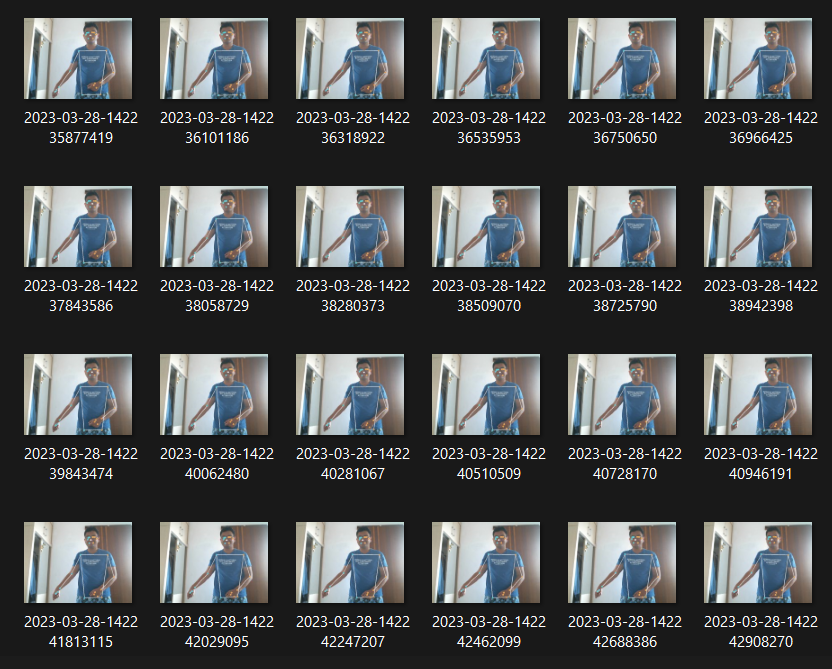
\includegraphics[width=0.7\linewidth]{gambar/citra_dataset.png}
	\captionof{figure}{Gambar dengan Dataset}
	\label{fig:Datasetraw}
\end{figure}

Dataset awal yang digunakan dalam penelitian ini terdiri dari gambar dan skeleton yang dikombinasikan. Dataset ini awalnya diperoleh melalui penggunaan MediaPipe, sebuah perangkat lunak yang mampu mengenali dan melacak landmark atau titik-titik penting pada objek gambar. Selanjutnya, dataset tersebut menjalani proses ekstraksi menggunakan program khusus yang telah dikembangkan dalam penelitian ini. Proses ekstraksi tersebut bertujuan agar bisa menghasilkan skeleton atau rangkaian titik-titik penting pada setiap gambar, dengan latar belakang yang diubah menjadi hitam supaya memudahkan analisis dan pemrosesan lebih lanjut. Hasil dari proses ekstraksi tersebut dapat dilihat dalam Gambar \ref{fig:Datasetekstark}, yang menunjukkan representasi visual dari skeleton yang dihasilkan dari dataset tersebut. Skeleton tersebut akan menjadi dasar dalam pembentukan dan pelatihan model CNN menjalankan tugas klasifikasi huruf pada Semaphore.

\begin{figure}[!hbt]
	\centering
	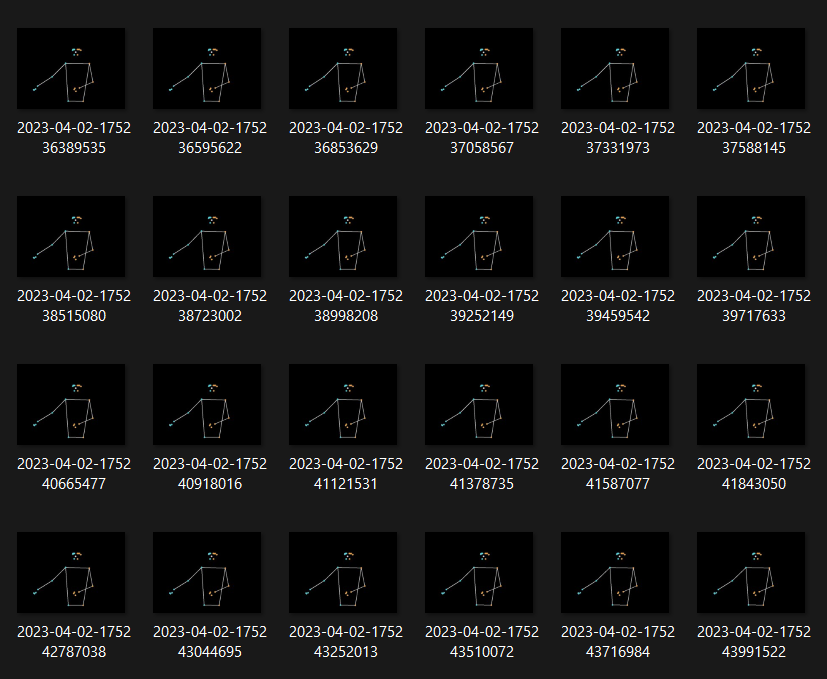
\includegraphics[width=0.7\linewidth]{gambar/tugas-akhir-dawe.png}
	\captionof{figure}{Gambar Hasil Ekstraksi Dataset}
	\label{fig:Datasetekstark}
\end{figure}

Dataset yang telah melalui proses ekstraksi tersebut kemudian digunakan sebagai \textit{input}  model-model deep learning yang digunakan dalam penelitian ini. Dataset ini digunakan sebagai cara melatih dan memvalidasi model-model deep learning yang akan digunakan dalam tugas klasifikasi huruf pada Semaphore. Dengan menggunakan dataset yang telah diekstrak, model-model deep learning dapat belajar dan mempelajari pola-pola penting dalam data, sehingga dapat melakukan prediksi yang akurat pada data yang belum pernah dilihat sebelumnya

\begin{table}[htbp]
	\centering
	\captionof{table}{Daftar Label}
	\label{tab:datasetlabel}
	\begin{tabular}{|c|c|c|c|c|}
		\hline
		A & B & C & D & E \\
		\hline
		F & G & H & I & J \\
		\hline
		K & L & M & N & O \\
		\hline
		P & Q & R & S & T \\
		\hline
		U & V & W & X & Y \\
		\hline
		Z &   Akhir &   &   &   \\
		\hline
	\end{tabular}
\end{table}

Tabel \ref{tab:datasetlabel} menampilkan huruf-huruf yang digunakan sebagai dataset dalam penelitian ini. Setiap huruf dalam dataset memiliki karakteristik unik dan bentuk yang tetap atau tidak mengalami perubahan. Huruf-huruf ini merupakan representasi visual dari alfabet yang sering digunakan dalam komunikasi dan penulisan. Dalam konteks tugas klasifikasi pada Semaphore, penting memahami dan mengenali setiap huruf dengan tepat. Oleh karena itu, dataset yang digunakan dalam penelitian ini mencakup seluruh huruf alfabet, termasuk huruf-huruf yang memiliki kurva, sudut, dan garis yang berbeda dalam bentuknya. Dengan memperhatikan bentuk yang statik dan tidak berubah dari setiap huruf dalam dataset, model CNN dapat belajar  mengenali pola visual yang khas dan membedakan satu huruf dari yang lainnya. Dataset yang mencakup variasi huruf ini memungkinkan model bisa melatih dirinya dalam mengenali dan mengklasifikasikan huruf-huruf dengan akurasi tinggi. Melalui penggunaan dataset yang terdiri dari huruf-huruf yang memiliki bentuk yang statik, penelitian ini bertujuan mengembangkan model CNN yang mampu mengenali huruf-huruf secara akurat. Dengan demikian, hasil evaluasi dan performa model dapat diukur dengan baik dalam tugas klasifikasi huruf pada Semaphore.

\section{Model CNN}
Awalnya, fungsi ini menerima parameter JumlahKelas yang menunjukkan jumlah kelas dalam dataset yang digunakan. Selanjutnya, dilakukan inisialisasi \textit{input} layer dengan ukuran (128, 128, 3), sesuai dengan dimensi gambar pada dataset.Setelahnya, dilakukan serangkaian operasi \textit{Conv2D} dan \textit{MaxPooling2D}. Terdapat tiga layer \textit{Conv2D} dengan masing-masing memiliki 32 \textit{neuron} dan \textit{filter} berukuran 3x3. Aktivasi \textit{ReLU} digunakan dalam mengaktifkan \textit{neuron}-\textit{neuron} tersebut. \textit{Padding} 'same' diterapkan agar ukuran \textit{output} tetap sama dengan \textit{input}. Setelah setiap layer \textit{Conv2D}, dilakukan \textit{MaxPooling2D} dengan ukuran \textit{pooling} 2x2 dan \textit{padding} 'same' dalam melakukan \textit{downsampling} dan mengurangi dimensi data.Kemudian, dilakukan layer \textit{Conv2D} lagi dengan 16 \textit{neuron} dan \textit{filter} berukuran 3x3, diikuti oleh \textit{MaxPooling2D} dengan ukuran \textit{pooling} 2x2 dan \textit{padding} 'same'. Langkah ini bertujuan dalam mengekstraksi fitur-fitur yang lebih kompleks dari data.Setelah melalui serangkaian operasi \textit{Conv2D} dan \textit{MaxPooling2D}, data kemudian diflatten menjadi vektor satu dimensi menggunakan layer Flatten. Hal ini diperlukan agar data dapat dimasukkan ke dalam layer \textit{Dense}, yaitu layer \textit{fully connected}.

Selanjutnya, data melewati layer \textit{Dense} dengan 16 \textit{neuron} yang menggunakan aktivasi \textit{ReLU}. Layer ini mempelajari pola-pola yang lebih kompleks dari data yang telah diekstraksi sebelumnya. dalam mencegah overfitting, terdapat layer Dropout dengan tingkat dropout sebesar 0.2.Selanjutnya, data melewati layer \textit{Dense} kembali dengan 16 \textit{neuron} dan aktivasi \textit{ReLU}. Layer ini memperkuat pembelajaran fitur-fitur yang relevan.Terakhir, data melewati layer \textit{Dense} dengan jumlah \textit{neuron} sesuai dengan JumlahKelas yang digunakan. Aktivasi \textit{softmax} digunakan sebagai cara mendapatkan probabilitas kelas pada \textit{output} layer. Model CNN ini dikompilasi dengan \textit{mean squared error} sebagai \textit{loss} function dan optimizer \textit{Adam}. Metrik akurasi juga digunakan dengan tujuan mengevaluasi performa model. Pada skenario ini, dilakukan pelatihan model selama 30 \textit{epoch}.

\subsection*{Performa dan Fungsionalitas Model CNN Skenario Pertama}
Grafik akurasi dari Model CNN Pertama, seperti yang ditunjukkan pada Gambar \ref{fig:AkurasiCNN1}, memberikan pemahaman awal yang penting dalam penelitian ini. Model ini mendasari skenario-skenario lain yang digunakan dalam penelitian dengan tujuan eksplorasi konfigurasi model CNN yang beragam dan mencari hasil optimal melalui tugas klasifikasi yang diberikan.

Dalam skenario ini, Model CNN Pertama terdiri dari empat layer \textit{Conv2D} yang diikuti oleh layer Maxpooling. Jumlah neuron pada setiap layer \textit{Conv2D} adalah 32, 32, 32, dan 16. Model ini dilatih selama 30 epoch, sehingga memungkinkan adaptasi yang cukup baik terhadap data pelatihan. Selain akurasi, grafik loss dari Model CNN Pertama, yang ditampilkan dalam Gambar \ref{fig:lossModelCNN1}, memberikan informasi penting tentang sejauh mana prediksi model mendekati nilai sebenarnya. Dalam penelitian ini, \textit{loss function} digunakan sebagai metrik sehingga dapat mengukur kesalahan prediksi model.

Grafik akurasi dan loss ini memberikan dasar yang kuat dalam pengembangan dan evaluasi skenario-skenario lain dalam penelitian ini. Dengan memvariasikan konfigurasi model CNN, diharapkan penelitian ini dapat menggali lebih dalam dan memperoleh hasil optimal yang memenuhi persyaratan klasifikasi yang diberikan.Pemahaman yang mendalam terhadap model dasar ini juga akan membantu dalam membandingkan dan mengevaluasi performa model-model lain yang dikembangkan dalam penelitian. Dengan melihat grafik-gambar tersebut, dapat diidentifikasi pola dan tren yang berpotensi memberikan wawasan berharga dalam mengoptimalkan model CNN yang mengerjakan tugas klasifikasi yang dihadapi. Hal ini perlu diperhatikan bahwa skenario-skenario lain dalam penelitian ini melibatkan modifikasi pada jumlah lapisan, ukuran \textit{filter}, aktivasi, atau penggunaan teknik seperti dropout atau regularisasi
\begin{figure}[!hbt]
	\centering
	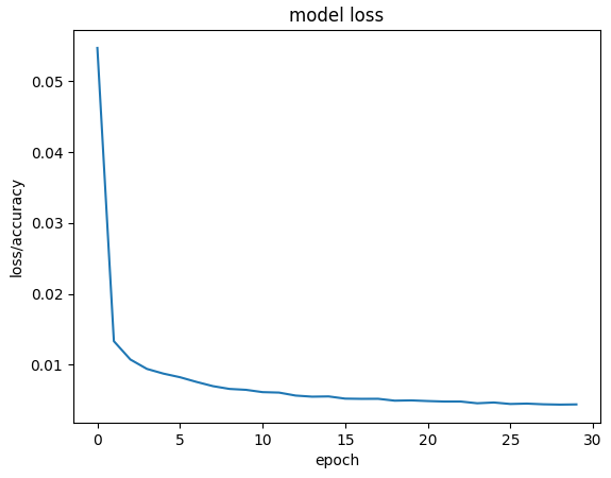
\includegraphics[width=0.7\linewidth]{gambar/bener/Loss_ModelCNN.png}
	\captionof{figure}{Loss Model CNN dengan epoch 30}
	\label{fig:lossModelCNN1}
\end{figure}
Berdasarkan Gambar \ref{fig:lossModelCNN1}. Pada \textit{Epoch} 1, \textit{loss} awal sebesar 0.0547 menunjukkan tingkat kesalahan yang cukup tinggi dalam mengklasifikasikan karakter. Namun, seiring berjalannya pelatihan, terjadi penurunan yang signifikan pada \textit{loss} pada setiap \textit{Epoch} berikutnya.Pada \textit{Epoch} 2 hingga \textit{Epoch} 8, terjadi penurunan yang cukup drastis pada \textit{loss} dari 0.0133 menjadi 0.00697. Periode ini menunjukkan peningkatan yang cepat dalam kemampuan model dalam meminimalkan kesalahan dalam mengklasifikasikan karakter. Penurunan yang signifikan ini dapat disebabkan oleh adanya pembelajaran dan penyesuaian parameter-model yang dilakukan oleh algoritma optimasi. Dari \textit{Epoch} 9 hingga \textit{Epoch} 15, penurunan \textit{loss} berlangsung dengan laju yang lebih lambat, menurun dari 0.00658 menjadi 0.00553. Pada tahap ini, model telah mencapai tingkat akurasi yang tinggi, sehingga perbaikan lebih lanjut dalam mengurangi \textit{loss} menjadi lebih sulit. Meskipun demikian, penurunan yang terjadi menunjukkan adanya peningkatan kemampuan model dalam mengenali dan mengklasifikasikan karakter.

Dalam periode \textit{Epoch} 16 hingga \textit{Epoch} 22, terjadi penurunan yang lebih kecil pada \textit{loss} dari 0.00521 menjadi 0.00481. Perubahan ini menunjukkan bahwa model telah mendekati batas kemampuan dalam mengurangi kesalahan. Pada tahap ini, fokus lebih pada \textit{fine-tuning} dari model sehingga meningkatkan generalisasi dan meminimalkan \textit{overfitting}. Dari \textit{Epoch} 23 hingga \textit{Epoch} 29, terlihat penurunan yang lebih lambat dan stabil dalam \textit{loss}, dari 0.00481 menjadi 0.00437. Pada tahap ini, model telah mencapai tingkat yang sangat rendah dalam mengurangi kesalahan dan menunjukkan kemampuannya dalam mengklasifikasikan karakter dengan tingkat akurasi yang tinggi. Pada \textit{Epoch} terakhir, yaitu \textit{Epoch} 30, \textit{loss} mencapai 0.00440. Meskipun terjadi penurunan yang lebih kecil dibandingkan beberapa \textit{Epoch} sebelumnya, hal ini menunjukkan bahwa model telah mencapai tingkat yang sangat baik dalam mengurangi kesalahan. \textit{Loss} yang rendah pada tahap ini mengindikasikan bahwa model telah berhasil mempelajari pola-pola yang ada pada data pelatihan dan mampu menggeneralisasi pada data yang belum pernah dilihat sebelumnya. Secara keseluruhan, perubahan loss dari Epoch ke Epoch tersebut menggambarkan adanya kemajuan dalam pelatihan model dan peningkatan kemampuan dalam mengklasifikasikan karakter. Penurunan loss yang stabil dan konsisten menunjukkan bahwa model tersebut mampu mengenali pola-pola penting pada data dan dapat menggeneralisasi dengan baik.


\begin{figure}[!hbt]
	\centering
	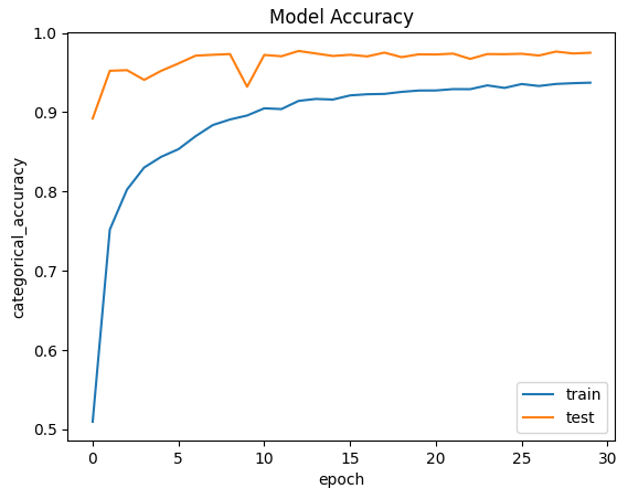
\includegraphics[width=0.7\linewidth]{gambar/bener/Accuracy_ModelCNN.png}
	\captionof{figure}{Akurasi Model CNN dengan epoch 30}
	\label{fig:AkurasiCNN1}
\end{figure}


Berdasarkan Gambar \ref{fig:AkurasiCNN1} , Pada \textit{Epoch} pertama, akurasi pelatihan sebesar 0.5093 menunjukkan performa awal yang rendah. Hal ini bisa disebabkan oleh inisialisasi acak parameter-model dan kurangnya pembelajaran pada tahap awal. Namun, hasil validasi akurasi sebesar 0.8920 menunjukkan bahwa model memiliki kemampuan dalam mengklasifikasikan karakter dengan tingkat keberhasilan yang lebih baik pada data yang belum pernah dilihat sebelumnya. Selama \textit{Epoch} 2 hingga \textit{Epoch} 8, terjadi peningkatan yang signifikan dalam akurasi pelatihan dari 0.7518 menjadi 0.8837. Hal ini menunjukkan bahwa model secara bertahap mempelajari pola-pola yang ada pada data pelatihan dan meningkatkan kemampuannya dalam mengklasifikasikan karakter. Validasi akurasi juga menunjukkan peningkatan yang konsisten, mencapai 0.9724 pada \textit{Epoch} 8. Dari \textit{Epoch} 9 hingga \textit{Epoch} 15, terlihat peningkatan yang lebih lambat dalam akurasi pelatihan dari 0.8907 menjadi 0.9159. Meskipun perubahan tersebut tidak signifikan, tetapi tetap menunjukkan adanya kemajuan dalam kemampuan model dalam mengenali karakter. Validasi akurasi tetap tinggi, mencapai 0.9709 pada \textit{Epoch} 15.

Pada periode \textit{Epoch} 16 hingga \textit{Epoch} 22, terjadi peningkatan yang stabil dalam akurasi pelatihan dari 0.9211 menjadi 0.9290. Meskipun perubahan tersebut tidak besar, tetapi menunjukkan bahwa model terus mengasah kemampuannya dalam mengklasifikasikan karakter dengan tingkat akurasi yang tinggi. Validasi akurasi juga tetap konsisten, mencapai 0.9738 pada \textit{Epoch} 22. Dari \textit{Epoch} 23 hingga \textit{Epoch} 29, akurasi pelatihan mencapai tingkat yang tinggi dan stabil, yaitu sekitar 0.9305 hingga 0.9372. Hal ini menunjukkan bahwa model telah mencapai titik jenuh dalam pembelajaran dan mampu mengklasifikasikan karakter dengan akurasi yang konsisten. Validasi akurasi tetap tinggi, mencapai 0.9765 pada \textit{Epoch} 28. 

Pada \textit{Epoch} terakhir, yaitu \textit{Epoch} 30, akurasi pelatihan mencapai 0.9372. Meskipun perubahan tersebut kecil, namun menunjukkan bahwa model telah mencapai tingkat kinerja yang sangat baik dalam mengklasifikasikan karakter. Validasi akurasi juga tetap tinggi, mencapai 0.9750, menunjukkan kemampuan model dalam menggeneralisasi pada data yang belum pernah dilihat sebelumnya.Secara keseluruhan, terlihat bahwa akurasi pelatihan dan validasi akurasi secara konsisten meningkat seiring dengan berjalannya proses pelatihan. Model berhasil mempelajari pola-pola yang ada pada data pelatihan dan dapat menggeneralisasi dengan baik pada data yang belum pernah dilihat sebelumnya. Hal ini menunjukkan bahwa model telah mencapai tingkat kinerja yang baik dalam mengklasifikasikan karakter. Perlu dicatat bahwa peningkatan akurasi yang terjadi pada tahap-tahap awal lebih signifikan daripada pada tahap-tahap akhir. Hal ini mengindikasikan bahwa model mencapai titik jenuh dalam pembelajaran pada tahap-tahap akhir.


\begin{figure}[!hbt]
	\centering
	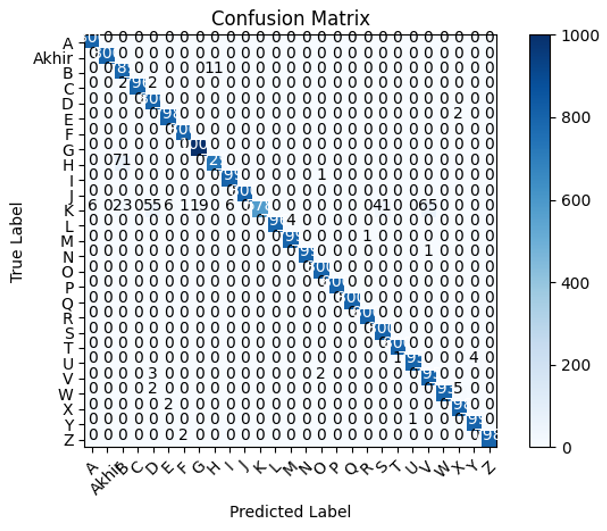
\includegraphics[width=0.7\linewidth]{gambar/bener/ConfusionMatrix_ModelCNN.png}
	\captionof{table}{Hasil Confusion Matriks Model CNN dengan epoch 30}
	\label{fig:TabelModelCNN1}
\end{figure}


Tabel \textit{Confusion Matrix} yang terlampir pada \ref{fig:TabelModelCNN1} adalah representasi visual dari hasil klasifikasi yang dilakukan pada dataset. \textit{Confusion Matrix} digunakan sebagai cara mengevaluasi kinerja model klasifikasi dengan membandingkan prediksi model dengan label sebenarnya. Tabel tersebut terdiri dari 27 baris dan 27 kolom yang mewakili label atau kelas yang ada dalam dataset.Pada setiap sel dalam tabel, angka yang tercantum menunjukkan jumlah sampel yang termasuk dalam kombinasi tertentu antara prediksi dan label sebenarnya. Misalnya, pada sel (A, A), angka 800 menunjukkan bahwa ada 800 sampel yang berhasil diklasifikasikan dengan benar sebagai kelas A. Begitu pula persebaran sel lainnya.Dalam analisis keseluruhan tabel \textit{Confusion Matrix}, Dapat ditinjau performa model klasifikasi setiap kelas secara rinci. Sebagai contoh, kelas A dan kelas Akhir berhasil diklasifikasikan dengan sempurna, tanpa adanya kesalahan prediksi. Namun, pada kelas B, terdapat 11 sampel yang seharusnya kelas B, namun salah diklasifikasikan sebagai kelas H. Kemudian, pada kelas C, ada 2 sampel yang salah diklasifikasikan sebagai kelas D dan 2 sampel lainnya salah diklasifikasikan sebagai kelas H. Sebaliknya, kelas D dan kelas E berhasil diklasifikasikan dengan sempurna tanpa kesalahan prediksi.

Bagi kelas lainnya, seperti kelas F, G, H, I, dan J, model juga berhasil mengklasifikasikan sampel dengan benar. Namun, terdapat kesalahan prediksi pada beberapa kelas, seperti kelas K, M, N, S, U, W, X, Y, dan Z. Dalam kasus tersebut, jumlah kesalahan prediksi dapat dilihat pada sel-sel yang bersesuaian dalam tabel \textit{Confusion Matrix}.Selain itu, terdapat temuan menarik terkait akurasi deteksi dan label huruf K. Dalam analisis tersebut, ditemukan bahwa akurasi deteksi dan label huruf K sebesar 578. Hal ini menunjukkan adanya kesalahan dalam dataset label huruf K yang mengakibatkan kesalahan dalam proses pelatihan model. Terdapat 185 data pelatihan yang seharusnya berisi huruf V, namun keliru dimasukkan sebagai huruf K. Kesalahan ini terjadi karena kesalahan dalam pengelompokan data ke dalam folder yang menyebabkan kesalahan dalam mengidentifikasi huruf K sebagai huruf V.

Efek dari kesalahan tersebut tampak pada hasil deteksi huruf K. Dalam kasus ini, terdapat 65 kasus di mana huruf K salah terdeteksi sebagai huruf V, 19 kasus sebagai huruf G, 23 kasus sebagai huruf B, dan 61 kasus sebagai huruf S. Hal ini menunjukkan adanya kebingungan dalam proses klasifikasi model, di mana model sulit membedakan antara huruf K dengan huruf-huruf lainnya yang memiliki kemiripan visual.Selain kesalahan pada label huruf K, terdapat juga beberapa kesalahan prediksi lainnya yang dapat dilihat dari nilai di luar diagonal utama pada \textit{Confusion Matrix}. Sebagai contoh, pada baris B dan kolom H terdapat 11 contoh yang seharusnya huruf B tetapi salah terklasifikasi sebagai huruf H. Hal ini menunjukkan bahwa terdapat kesulitan dalam membedakan antara huruf B dan huruf H dalam proses klasifikasi.Dengan mengevaluasi dan menganalisis \textit{Confusion Matrix} ini, Dapat diidentifikasi jenis kesalahan yang umum terjadi dalam model klasifikasi huruf. Informasi ini penting dalam memahami kelemahan model dan mengembangkan strategi perbaikan yang lebih baik, seperti peningkatan kualitas dataset atau penyesuaian model dalam mengatasi kesalahan yang spesifik.


Tabel evaluasi metrik pada Tabel \ref{tab:tabelevaluasicnn} menggambarkan hasil analisis performa sistem klasifikasi terhadap berbagai kelas atau label yang dievaluasi pada Model CNN. Metrik-metrik yang digunakan dalam tabel ini adalah Precision, Recall, dan F1-Score, yang merupakan indikator penting dalam mengukur ketepatan dan keberhasilan sistem dalam melakukan klasifikasi.
\begin{table}
	\centering
	\caption{Tabel Evaluasi Metrik Model CNN}
	\begin{tabular}{|c|c|c|c|c|}
	\hline
	Class & Precision & Recall & F1-score \\
	\hline
	A     & 0.992556  & 1.00000 & 0.996264 \\
	Akhir & 0.990099  & 1.00000 & 0.995025 \\
	B     & 0.920653  & 0.98625 & 0.952323 \\
	C     & 1.000000  & 0.99500 & 0.997494 \\
	D     & 0.917431  & 1.00000 & 0.956938 \\
	E     & 0.991304  & 0.99750 & 0.994393 \\
	F     & 0.996264  & 1.00000 & 0.998129 \\
	G     & 0.971817  & 1.00000 & 0.985707 \\
	H     & 0.985135  & 0.91125 & 0.946753 \\
	I     & 0.992547  & 0.99875 & 0.995639 \\
	J     & 1.000000  & 1.00000 & 1.000000 \\
	K     & 1.000000  & 0.58750 & 0.740157 \\
	L     & 1.000000  & 0.99500 & 0.997494 \\
	M     & 0.995019  & 0.99875 & 0.996881 \\
	N     & 1.000000  & 0.99875 & 0.999375 \\
	O     & 0.993789  & 1.00000 & 0.996885 \\
	P     & 1.000000  & 1.00000 & 1.000000 \\
	Q     & 1.000000  & 1.00000 & 1.000000 \\
	R     & 0.985222  & 1.00000 & 0.992556 \\
	S     & 0.940071  & 1.00000 & 0.969110 \\
	T     & 0.998752  & 1.00000 & 0.999375 \\
	U     & 0.998744  & 0.99375 & 0.996241 \\
	V     & 0.841270  & 0.99375 & 0.911175 \\
	W     & 0.993734  & 0.99125 & 0.992491 \\
	X     & 0.991272  & 0.99375 & 0.992509 \\
	Y     & 0.995019  & 0.99875 & 0.996881 \\
	Z     & 1.000000  & 0.99750 & 0.998748 \\
	\hline
	\end{tabular}
	\label{tab:tabelevaluasicnn}
	\end{table}
\textit{Precision}, yang merupakan rasio antara \textit{true positive} dan semua objek yang diklasifikasikan sebagai positif, menggambarkan sejauh mana sistem dapat mengidentifikasi positif sejati dengan akurat. Dalam tabel, nilai \textit{Precision} berkisar dari 0.841 hingga 1.000. Nilai \textit{Precision} yang mendekati 1.000, seperti yang terlihat pada kelas A, C, F, J, N, P, Q, dan Z, menandakan sistem memiliki kemampuan yang sangat baik dalam mengenali positif sejati, dengan sangat sedikit \textit{false positive}.

Sementara itu, \textit{Recall} adalah rasio antara \textit{true positive} dan semua objek yang benar-benar positif, yang mencerminkan kemampuan sistem dalam mengenali seluruh data positif yang ada. Hasil dari tabel menunjukkan bahwa nilai \textit{Recall} juga bervariasi, dengan rentang nilai antara 0.587 hingga 1.000. Kelas dengan nilai \textit{Recall} mendekati 1.000, seperti pada kelas A, Akhir, D, F, G, J, O, P, dan Q, menandakan sistem mampu mengidentifikasi hampir seluruh data positif yang ada.

Selanjutnya, \textit{F1-Score} digunakan sebagai indikator keseluruhan kualitas performa sistem klasifikasi dengan mempertimbangkan kedua metrik sebelumnya. \textit{F1-Score} dihitung sebagai harmonisasi dari \textit{Precision} dan \textit{Recall}, memberikan gambaran tentang sejauh mana sistem mampu mencapai keseimbangan yang baik antara \textit{Precision} dan \textit{Recall}. Nilai \textit{F1-Score} berkisar antara 0.740 hingga 1.000, dengan kelas-kelas seperti A, C, F, J, N, P, Q, dan Z memiliki \textit{F1-Score} tinggi, menandakan keseimbangan yang baik dalam performa klasifikasi.

Selanjutnya, hasil rata-rata dari \textit{Precision}, \textit{Recall}, dan \textit{F1-Score} dihitung seluruh kelas yang dievaluasi. Rata-rata \textit{Precision} sekitar 0.973, yang mengindikasikan tingkat akurasi yang tinggi dalam mengenali positif sejati secara keseluruhan. Rata-rata \textit{Recall} sekitar 0.809, menunjukkan kemampuan sistem yang baik dalam mengenali seluruh data positif. Sementara rata-rata \textit{F1-Score} sekitar 0.881, menandakan bahwa sistem klasifikasi mampu mencapai keseimbangan yang baik antara \textit{Precision} dan \textit{Recall} secara keseluruhan.

Penting dicatat bahwa performa suatu sistem klasifikasi dapat berbeda-beda bagi setiap kelas, tergantung pada kompleksitas dan perwakilan data dari masing-masing kelas. Oleh karena itu, analisis metrik ini memberikan wawasan yang berharga bagi para peneliti dan praktisi dalam mengevaluasi performa sistem secara menyeluruh dan mengidentifikasi kelas-kelas yang memerlukan perbaikan lebih lanjut.

Dari hasil analisis, dapat disimpulkan bahwa sistem klasifikasi memiliki performa yang baik dalam mengenali positif sejati dan mencapai keseimbangan yang memadai antara \textit{Precision} dan \textit{Recall} pada kelas-kelas tertentu. Namun, terdapat beberapa kelas dengan nilai metrik yang perlu ditingkatkan guna meningkatkan akurasi dan efektivitas sistem. Hasil evaluasi metrik ini dapat digunakan sebagai acuan dalam mengoptimalkan performa sistem klasifikasi, mengidentifikasi aspek yang perlu diperbaiki, dan meningkatkan kualitas klasifikasi pada berbagai bidang aplikasi.

\section{Model CNN Kedua}
Pada Model CNN Kedua , Dataset tersebut melewati beberapa lapisan yang berfungsi sebagai metode mengekstraksi fitur. Pertama, dataset melewati lapisan \textit{Conv2D} dengan 32 \textit{neuron}, \textit{filter} 3x3, aktivasi \textit{ReLU}, dan \textit{padding} yang sama. Kemudian, dilakukan \textit{MaxPooling2D} dengan ukuran \textit{pooling} 2x2 dan \textit{padding} yang sama. Selanjutnya, dataset melewati lapisan \textit{Conv2D} lain dengan 16 \textit{neuron}, \textit{filter} 3x3, aktivasi \textit{ReLU}, dan \textit{padding} yang sama sebanyak dua kali. Kemudian dilakukan lagi \textit{MaxPooling2D} dengan ukuran \textit{pooling} 2x2 dan \textit{padding} yang sama. Dan diakhiri dengan dataset melewati lapisan \textit{Conv2D} dengan 8 \textit{neuron} , \textit{filter} 3x3 , aktivasi \textit{ReLU} dan \textit{padding} yang sama sebanyak dua kali serta \textit{MaxPooling2D} dengan ukuran \textit{pooling} 2x2 

Setelah proses ekstraksi fitur, dataset kemudian masuk ke tahap klasifikasi. Pertama, dilakukan flattening agar mengubah data menjadi vektor satu dimensi. Kemudian, data melewati lapisan \textit{Dense} dengan 16 \textit{neuron} dan aktivasi \textit{ReLU}. Supaya mencegah overfitting, dilakukan dropout dengan dropout rate 0.2. Setelah itu, terdapat lapisan \textit{Dense} lagi dengan 16 \textit{neuron} dan aktivasi \textit{ReLU}. Lapisan terakhir menggunakan \textit{Dense} dengan jumlah \textit{neuron} sesuai dengan jumlah kelas pada dataset (JumlahKelas) dan aktivasi \textit{softmax} supaya menghasilkan \textit{output} probabilitas kelas. Model CNN ini menggunakan fungsi \textit{loss} \textit{mean squared error} dan optimizer \textit{Adam} dalam proses kompilasi Grafik akurasi dari Model CNN Kedua tersedia di Gambar \ref{fig:AkurasiCNNKedua}. Dalam skenario ini, terdapat empat lapisan \textit{Conv2D} yang diikuti oleh \textit{Maxpooling}. Jumlah \textit{neuron} dalam setiap lapisan \textit{Conv2D} adalah 32, 16, 16, dan 8. Model CNN ini dilatih selama 30\textit{ epoch}.

Grafik \textit{loss} dari Model CNN Kedua dapat ditemukan di Gambar \ref{fig:lossModelCNNKedua}. \textit{Loss} function digunakan sebagai cara mengukur sejauh mana prediksi model CNN mendekati nilai sebenarnya. Pada skenario ini, model CNN berhasil mengurangi \textit{loss} secara signifikan selama proses pelatihan selama 30\textit{ epoch}.

\begin{figure}[!hbt]
	\centering
	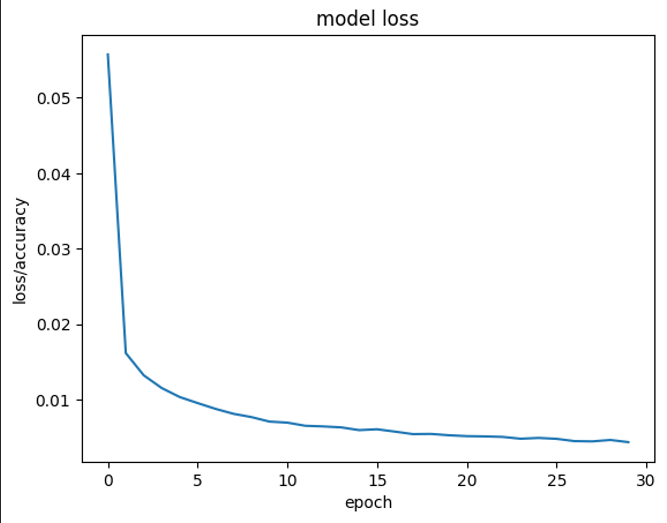
\includegraphics[width=0.7\linewidth]{gambar/bener/Loss_ModelCNN2.png}
	\captionof{figure}{Loss Model CNN 2 dengan epoch 30}
	\label{fig:lossModelCNNKedua}
\end{figure}

Pada analisis \textit{Loss} dari Model CNN 2, terlihat bahwa terjadi penurunan yang signifikan dalam nilai \textit{loss} seiring dengan peningkatan \textit{epoch}. Hal ini menunjukkan bahwa model secara bertahap mampu mengurangi kesalahan prediksi dan meningkatkan akurasi dalam proses pelatihan. Awalnya, pada \textit{epoch} pertama, \textit{loss} memiliki nilai 0.0557, namun melalui pelatihan yang berkelanjutan, model berhasil mengurangi nilai \textit{loss} menjadi 0.0043 pada \textit{epoch} ke-30.Ketika melihat kurva \textit{loss}, terdapat fluktuasi pada beberapa \textit{epoch} awal, seperti pada \textit{epoch} kedua yang mengalami peningkatan. Namun, model mampu menyesuaikan bobotnya dengan baik dan secara konsisten menunjukkan penurunan \textit{loss} yang stabil seiring berjalannya waktu. Pada \textit{epoch} ke-15, model mencapai tingkat stabil dan kemampuan optimalisasi yang baik, di mana perubahan nilai \textit{loss} menjadi lebih kecil dan mendekati batas kemampuan model dalam pembelajaran.

Meskipun terdapat fluktuasi kecil pada beberapa \textit{epoch} terakhir, seperti pada \textit{epoch} ke-28, ke-29, dan ke-30, pola umum penurunan \textit{loss} tetap terjaga. Hal ini menunjukkan bahwa model CNN 2 telah mencapai tingkat konvergensi yang baik dan mampu memperbaiki prediksi dengan mengurangi kesalahan dalam proses pelatihan. Analisis \textit{loss} merupakan langkah awal yang penting dalam mengevaluasi performa model CNN 2. Dari hasil analisis ini, dapat disimpulkan bahwa model ini mampu mengurangi kesalahan prediksi secara konsisten dan meningkatkan performa dalam tugas klasifikasi huruf pada Semaphore. Dengan adanya penurunan \textit{loss} yang terjadi seiring berjalannya \textit{epoch}, model ini menunjukkan kemampuan yang baik dalam mengoptimalkan pembelajarannya dan memperbaiki prediksi yang dilakukan.

\begin{figure}[!hbt]
	\centering
	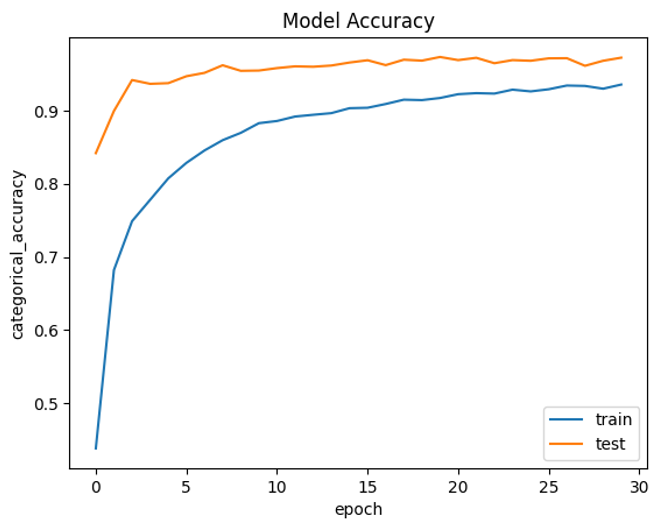
\includegraphics[width=0.7\linewidth]{gambar/bener/Accuracy_ModelCNN2.png}
	\captionof{figure}{Akurasi Model CNN 2 dengan epoch 30}
	\label{fig:AkurasiCNNKedua}
\end{figure}

Dalam analisis Akurasi dan Validasi Akurasi dari Model CNN 2 sesuai dengan Gambar \ref{fig:AkurasiCNNKedua}, terlihat adanya peningkatan yang signifikan dalam performa model sepanjang proses pelatihan. Pada awalnya, model memiliki Akurasi sebesar 43.85\% pada \textit{epoch} pertama. Namun, melalui iterasi pelatihan yang berkelanjutan, model berhasil mencapai tingkat Akurasi sebesar 93.53\% pada \textit{epoch} ke-30. Setiap \textit{epoch} menunjukkan perbaikan yang konsisten dalam Akurasi model. Dengan setiap siklus pelatihan, model semakin terlatih dalam mengklasifikasikan huruf-huruf pada Semaphore dengan lebih akurat. Validasi Akurasi juga mengalami peningkatan yang signifikan dari 84.17\% pada \textit{epoch} pertama menjadi 97.20\% pada \textit{epoch} ke-30. Analisis kurva Akurasi dan Validasi Akurasi menggambarkan tren yang positif sepanjang proses pelatihan. Walaupun terjadi fluktuasi kecil pada beberapa \textit{epoch}, seperti pada \textit{epoch} ke-11, ke-14, dan ke-21, namun secara keseluruhan, kenaikan Akurasi terus terjadi. Hal ini menunjukkan bahwa model mampu mempelajari pola-pola penting dari data pelatihan dan mampu menggeneralisasi dengan baik pada data baru.

Dengan mencapai tingkat Akurasi yang tinggi pada data pelatihan dan validasi, dapat disimpulkan bahwa model CNN 2 berhasil mengklasifikasikan huruf-huruf pada Semaphore dengan akurasi yang memuaskan. Keberhasilan model ini menunjukkan bahwa ia mampu memahami dan mengenali pola-pola yang ada pada dataset, sehingga mampu memberikan hasil prediksi yang akurat.Selain itu, perhatikan juga bahwa semakin tinggi Akurasi dan Validasi Akurasi yang dicapai oleh model, semakin baik pula kemampuannya dalam mengklasifikasikan huruf-huruf pada Semaphore. Tingkat Akurasi yang tinggi menunjukkan bahwa model mampu mengenali dan mempelajari fitur-fitur yang relevan dari dataset. Hal ini berdampak positif pada kemampuan model dalam menggeneralisasi dan mengaplikasikan pengetahuan yang telah dipelajari pada data baru. Melalui analisis Akurasi dan Validasi Akurasi yang telah dilakukan, dapat disimpulkan bahwa model CNN 2 berhasil mencapai performa yang baik dalam mengklasifikasikan huruf-huruf pada Semaphore. Tingkat Akurasi yang tinggi dan peningkatan yang konsisten selama proses pelatihan menunjukkan kemampuan model dalam mengenali pola-pola penting dari data. Dengan begitu, model ini memiliki potensi digunakan dalam aplikasi yang melibatkan pengenalan dan klasifikasi huruf-huruf pada Semaphore.

\begin{figure}[!hbt]
	\centering
	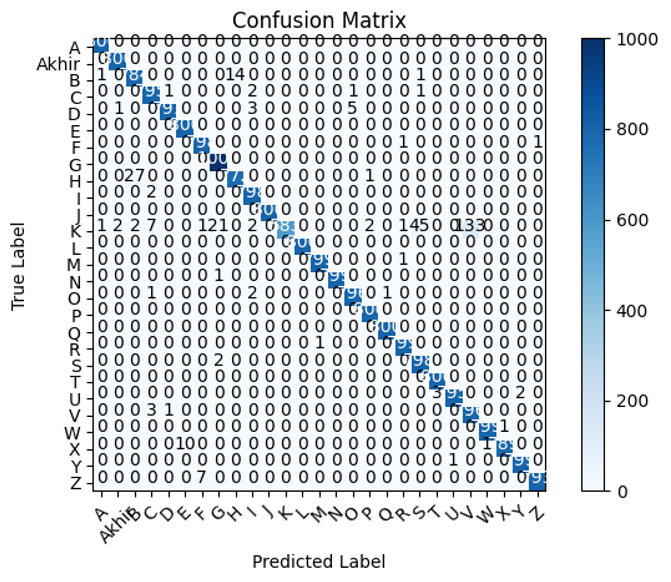
\includegraphics[width=0.7\linewidth]{gambar/bener/ConfusionMatrix_ModelCNN2.png}
	\captionof{table}{Hasil Confusion Matriks Model CNN Kedua dengan epoch 30}
	\label{fig:TabelModelCNNKedua}
\end{figure}

Gambar \textit{Confusion Matrix} Model CNN2 pada Gambar \ref{fig:TabelModelCNNKedua} memberikan gambaran tentang sejauh mana model mampu mengklasifikasikan setiap huruf dengan benar. Setiap sel pada gambar menunjukkan jumlah prediksi yang diberikan oleh model setiap kombinasi kelas sebenarnya dan prediksi. Pada gambar \textit{Confusion Matrix} ini, masing-masing huruf dari A hingga Z terdapat pada baris dan kolom yang terpisah. Setiap sel pada gambar menunjukkan jumlah prediksi yang dilakukan oleh model setiap kombinasi huruf yang berbeda. Misalnya, angka 800 pada baris A dan kolom A menunjukkan bahwa model dengan benar mengklasifikasikan huruf 'A' sebanyak 800 kali. Analisis Confusion Matrix memberikan wawasan yang sangat berharga terkait dengan performa model CNN 2 dalam mengklasifikasikan huruf-huruf pada Semaphore. Tujuannya mengevaluasi akurasi prediksi model secara mendalam serta mengidentifikasi pola dan kesalahan yang terjadi dalam proses pengenalan huruf-huruf tersebut. Melalui gambar Confusion Matrix yang terperinci, Dapat dilihat hasil prediksi yang spesifik bagi setiap huruf. Tidak hanya itu, melalui metrik evaluasi seperti precision, recall, dan f1-score, juga bisa memperoleh informasi yang berguna mengenai seberapa baik model mampu mengenali dan membedakan huruf-huruf tersebut.

Dalam analisis ini, ditemukan beberapa hal menarik yang patut diperhatikan. Misalnya, huruf-huruf seperti 'A', 'Akhir', 'E', dan 'G' menunjukkan tingkat akurasi yang tinggi, dengan nilai precision, recall, dan f1-score yang mendekati 1. Hal ini menandakan bahwa model mampu mengklasifikasikan huruf-huruf tersebut dengan sangat baik dan konsisten. Namun, di sisi lain, terdapat beberapa huruf yang menunjukkan tingkat akurasi yang relatif lebih rendah. Contohnya, huruf 'K' memiliki nilai precision yang sempurna (1.0), namun recall-nya masih tergolong rendah, menandakan adanya kesulitan dalam membedakan huruf ini dari huruf lainnya. Oleh karena itu, tujuan utama dari penelitian ini adalah agar meningkatkan akurasi dan mengatasi perbedaan antara huruf 'K' dengan huruf lainnya. Selain huruf 'K', beberapa huruf lain seperti 'B', 'D', 'H', 'O', 'S', 'U', dan 'V' juga menunjukkan tingkat akurasi yang relatif rendah, menandakan kesulitan dalam mengklasifikasikan huruf-huruf tersebut secara akurat. Dalam hal ini, penelitian ini bertujuan supaya bisa mengembangkan strategi baru atau mempertimbangkan penambahan fitur tambahan guna meningkatkan akurasi dalam pengenalan huruf-huruf tersebut. Selain aspek peningkatan akurasi, analisis Confusion Matrix juga mengungkapkan kasus menarik di mana huruf 'K' sering kali terbaca sebagai huruf 'V'. Hal ini mungkin disebabkan oleh kesalahan dalam proses labeling atau pengelompokan dataset, di mana dataset huruf 'V' secara tidak sengaja termasuk ke dalam folder yang semestinya berisi dataset huruf 'K'. Oleh karena itu, tujuan penelitian ini adalah melakukan perbaikan dalam pengelompokan dataset, sehingga model dapat mempelajari karakteristik dan pola yang lebih baik dalam membedakan antara huruf-huruf tersebut dengan akurasi yang lebih tinggi.

Secara keseluruhan, analisis Gambar Confusion Matrix memberikan pemahaman mendalam tentang performa Model CNN 2 dalam mengenali huruf-huruf pada Semaphore. Dengan memperhatikan metrik evaluasi dan pola-pola yang terlihat dalam tabel, penelitian ini bertujuan meningkatkan akurasi dan kemampuan model dalam mengklasifikasikan huruf-huruf dengan tepat dan akurat, serta mengatasi perbedaan yang mungkin terjadi antara huruf-huruf tertentu. Dengan demikian, tabel Confusion Matrix ini memberikan pemahaman yang lebih rinci tentang performa Model CNN 2 dalam mengklasifikasikan huruf-huruf pada Semaphore. Meskipun model memiliki tingkat akurasi yang tinggi secara keseluruhan, analisis Confusion Matrix membantu mengidentifikasi area yang memerlukan perbaikan lebih lanjut dan memberikan wawasan yang berguna dalam mengoptimalkan model.

Tabel evaluasi metrik pada Tabel \ref{tab:tabelevaluasicnn2} menyajikan hasil analisis performa sistem klasifikasi  berbagai kelas atau label yang dievaluasi. Metrik utama yang digunakan dalam analisis ini meliputi Precision, Recall, dan F1-Score, yang memberikan wawasan yang mendalam mengenai ketepatan dan keberhasilan sistem dalam melakukan klasifikasi pada setiap kelas.
\begin{table}[h]
	\centering
	\caption{Tabel Evaluasi Metrik CNN2}
	\begin{tabular}{|c|c|c|c|c|}
	\hline
	Class & Precision & Recall & F1-score \\
    \hline
	A & 0.997506 & 1.00000 & 0.998752 \\
	Akhir & 0.996264 & 1.00000 & 0.998129 \\
	B & 0.915888 & 0.98000 & 0.946860 \\
	C & 0.983911 & 0.99375 & 0.988806 \\
	D & 0.980173 & 0.98875 & 0.984443 \\
	E & 0.992556 & 1.00000 & 0.996264 \\
	F & 0.990074 & 0.99750 & 0.993773 \\
	G & 0.974659 & 1.00000 & 0.987167 \\
	H & 0.975000 & 0.68250 & 0.802941 \\
	I & 0.950000 & 0.99750 & 0.973171 \\
	J & 1.000000 & 1.00000 & 1.000000 \\
	K & 1.000000 & 0.59375 & 0.745098 \\
	L & 1.000000 & 1.00000 & 1.000000 \\
	M & 0.998750 & 0.99875 & 0.998750 \\
	N & 1.000000 & 0.99875 & 0.999375 \\
	O & 0.892377 & 0.99500 & 0.940898 \\
	P & 0.984010 & 1.00000 & 0.991940 \\
	Q & 0.998752 & 1.00000 & 0.999375 \\
	R & 0.996259 & 0.99875 & 0.997503 \\
	S & 0.941038 & 0.99750 & 0.968447 \\
	T & 0.977995 & 1.00000 & 0.988875 \\
	U & 0.998744 & 0.99375 & 0.996241 \\
	V & 0.770571 & 0.99500 & 0.868522 \\
	W & 0.968485 & 0.99875 & 0.983385 \\
	X & 0.998731 & 0.98375 & 0.991184 \\
	Y & 0.996259 & 0.99875 & 0.997503 \\
	Z & 0.998741 & 0.99125 & 0.994981 \\
	\hline
	\end{tabular}
	\label{tab:tabelevaluasicnn2}
	\end{table}
\textit{Precision} menggambarkan sejauh mana sistem dapat mengenali positif sejati secara akurat dari seluruh data yang diklasifikasikan sebagai positif. Tabel tersebut menunjukkan bahwa sistem memiliki tingkat \textit{Precision} yang tinggi pada kelas A, Akhir, E, F, J, M, N, P, Q, R, Y, dan Z, dengan nilai \textit{Precision} mendekati atau bahkan mencapai 1.00. Hal ini menandakan bahwa sistem mampu mengidentifikasi data positif yang relevan dengan sangat tepat dari seluruh data yang diklasifikasikan sebagai positif.

Sementara itu, \textit{Recall} mengukur kemampuan sistem dalam mengenali seluruh data positif yang ada dari seluruh data positif yang sebenarnya. Beberapa kelas, seperti A, Akhir, E, F, G, J, M, N, O, P, Q, R, S, T, dan Z, memiliki nilai \textit{Recall} yang mendekati atau bahkan mencapai 1.00, menunjukkan bahwa sistem memiliki kemampuan yang baik dalam mengenali sebagian besar atau bahkan seluruh data positif yang ada. F1-Score, sebagai harmonisasi antara \textit{Precision} dan \textit{Recall}, memberikan gambaran menyeluruh tentang performa sistem klasifikasi. Beberapa kelas yang memiliki F1-Score tinggi adalah A, Akhir, E, F, J, M, N, P, Q, R, Y, dan Z, menandakan bahwa sistem mencapai keseimbangan yang optimal antara kemampuan mengenali positif sejati dan menghindari kesalahan klasifikasi.

Terkait rata-rata \textit{Precision} dari seluruh kelas, angka yang tercatat adalah sekitar 0.968, menunjukkan performa akurat sistem dalam mengenali positif sejati secara keseluruhan. Rata-rata \textit{Recall} sekitar 0.946, menandakan bahwa sistem memiliki kemampuan yang baik dalam mengenali sebagian besar data positif yang ada. Sedangkan rata-rata F1-Score sekitar 0.952, mengindikasikan keseimbangan yang baik antara \textit{Precision} dan \textit{Recall} secara keseluruhan . Dari hasil analisis tersebut, dapat disimpulkan bahwa sistem klasifikasi menunjukkan kinerja yang sangat baik dalam mengenali positif sejati dan mencapai keseimbangan optimal antara Precision dan Recall pada sejumlah kelas. Meskipun begitu, masih terdapat beberapa kelas dengan nilai metrik yang memerlukan peningkatan guna meningkatkan akurasi dan efektivitas sistem. Evaluasi metrik ini menjadi pijakan penting dalam pengembangan dan penyempurnaan sistem klasifikasi guna meningkatkan kualitas serta utilitasnya dalam berbagai bidang aplikasi.

\section{Model CNN ResNet50v2}
ModelCNN \textit{ResNet50V2} merupakan sebuah arsitektur \textit{Convolutional Neural Network (CNN)} yang menggunakan \textit{ResNet50V2} sebagai komponen utamanya berfungsi melakukan klasifikasi pada dataset dengan jumlah kelas yang telah ditentukan. Dalam proses pembuatannya, langkah-langkah berikut yang dilakukan sebagai cara mengatur dan mengoptimalkan model tersebut. Pertama, model menggunakan arsitektur \textit{ResNet50V2} sebagai basisnya. Arsitektur ini telah dilatih sebelumnya dengan menggunakan dataset \textit{ImageNet}, yang mengandung berbagai kategori gambar. Dengan menggunakan basis yang telah dilatih ini, model dapat memanfaatkan pengetahuan visual yang telah dipelajari pada tahap awal.

Selanjutnya, base model \textit{ResNet50V2} diset agar tidak dilatih ulang (trainable=False). Hal ini dilakukan sebagai cara menjaga agar bobot dan parameter dari base model tetap sama seperti yang telah dipelajari pada dataset \textit{ImageNet}. Dengan begitu, model tidak akan menghapus pengetahuan yang telah ada. Kemudian, \textit{output} dari base model dilakukan proses \textit{Global Average Pooling}. Langkah ini mengambil rata-rata dari setiap fitur yang dihasilkan oleh base model. Hasilnya adalah vektor fitur yang merepresentasikan gambar secara lebih kompak dan mengandung informasi penting terkait klasifikasi. Selanjutnya, vektor fitur tersebut diteruskan ke beberapa lapisan\textit{ Dense (fully-connected)}. Dalam model ini, terdapat dua lapisan\textit{ Dense} dengan fungsi aktivasi ReLU. Fungsi aktivasi ini membantu dalam memperkenalkan non-linearitas pada model. Selain itu, terdapat juga lapisan Dropout dengan nilai dropout sebesar 0.4. Lapisan Dropout digunakan sebagai upaya mengurangi overfitting dengan secara acak mengabaikan sebagian unit/neuron pada lapisan sebelumnya.Lapisan\textit{ Dense} terakhir memiliki jumlah neuron yang sesuai dengan jumlah kelas yang ditentukan. Fungsi aktivasi yang digunakan adalah softmax, yang menghasilkan probabilitas bagi setiap kelas. Dengan menggunakan softmax, model dapat memberikan prediksi kelas yang paling mungkin bagi suatu gambar.

Model \textit{CNN} \textit{ResNet50V2} ini kemudian dikompilasi dengan menggunakan \textit{loss function} berupa \textit{mean squared error (mse)}. \textit{Loss function} ini digunakan dalam mengukur seberapa baik prediksi model sesuai dengan nilai sebenarnya. \textit{Optimizer} yang digunakan adalah \textit{Adam}, yang merupakan algoritma optimisasi yang populer dalam melatih model \textit{neural network}.Dalam enam langkah tersebut, Model\textit{CNN} \textit{ResNet50V2} berhasil dibangun dengan menggunakan arsitektur \textit{ResNet50V2} sebagai basisnya, dilanjutkan dengan proses \textit{pooling} dan lapisan\textit{ Dense} yang menghasilkan probabilitas kelas. Model ini dapat dioptimalkan dengan mengatur \textit{hyperparameter} seperti \textit{dropout rate}, \textit{l2 regularization}, dan \textit{learning rate} pada \textit{optimizer}. Dengan konfigurasi ini, model siap  dilatih dengan data latih dan digunakan sebagai upaya klasifikasi pada dataset dengan jumlah kelas yang ditentukan

\subsection*{Performa dan Fungsionalitas Model CNN \textit{ResNet50v2} Skenario Pertama}

Grafik akurasi yang terkait dengan Model \textit{CNN} \textit{ResNet50V2} telah disajikan pada Gambar \ref{fig:AkurasiCNNResNet50V2}. Dalam skenario ini, model \textit{CNN} menggunakan arsitektur \textit{ResNet50V2} sebagai basisnya. Proses pelatihan model \textit{CNN} ini berlangsung selama 30 \textit{epoch}, yang mewakili jumlah iterasi yang dilakukan dalam melatih model. Penting diketahui bahwa grafik akurasi pada Gambar \ref{fig:AkurasiCNNResNet50V2} menunjukkan perkembangan performa model seiring dengan peningkatan jumlah \textit{epoch}. Pada awal pelatihan, akurasi mungkin masih rendah, tetapi seiring berjalannya waktu dan iterasi, model mengalami peningkatan akurasi yang signifikan. Hal ini menunjukkan bahwa model \textit{CNN} \textit{ResNet50V2} mampu mempelajari pola-pola penting dalam data latih dan menghasilkan prediksi yang semakin akurat. Selain itu, perlu dicatat bahwa grafik \textit{loss} pada Gambar \ref{fig:lossModelCNNResNet50v2} juga memberikan gambaran tentang kinerja model \textit{CNN} ResNet50V2. \textit{Loss} function digunakan sebagai metrik pengukuran seberapa baik model mendekati nilai sebenarnya dalam proses pelatihan. Dalam kasus ini, grafik \textit{loss} menunjukkan penurunan yang konsisten selama 30 \textit{epoch} pelatihan.

\begin{figure}[!hbt]
	\centering
	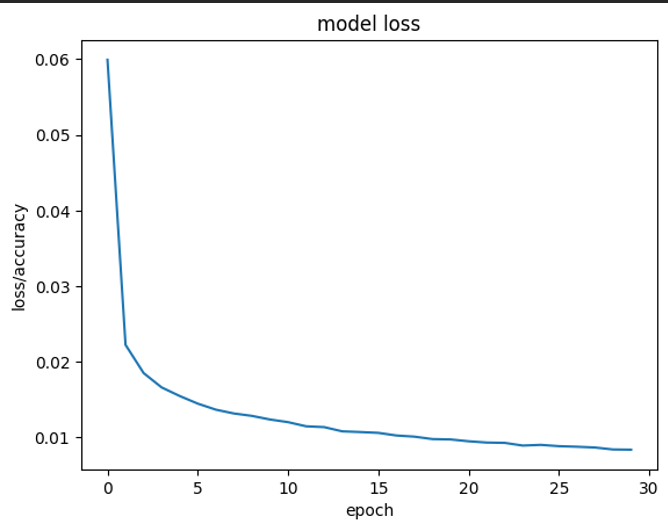
\includegraphics[width=0.7\linewidth]{gambar/bener/Loss_ModelCNNResNet50V2.png}
	\captionof{figure}{Loss Model CNN ResNet50V2 dengan epoch 30}
	\label{fig:lossModelCNNResNet50v2}
\end{figure}

Analisis terhadap data akurasi dan validasi akurasi Model CNN \textit{ResNet50V2} yang terletak pada Gambar \ref{fig:lossModelCNNResNet50v2} menunjukkan perubahan performa model selama proses pelatihan. Pada awal pelatihan, akurasi model terhadap data latih memiliki nilai rendah, yaitu 0.31339 pada \textit{epoch} pertama. Namun, seiring berjalannya iterasi pelatihan, terjadi peningkatan yang signifikan dalam akurasi model. Pada \textit{epoch} kedua, terjadi peningkatan yang cukup besar dalam akurasi model menjadi 0.59004 . Penurunan nilai \textit{loss} ini menunjukkan kemampuan model dalam mempelajari pola-pola penting dalam data latih dan meningkatkan akurasi prediksi. Perubahan ini juga mencerminkan efektivitas model dalam menyesuaikan bobot dan parameter selama pelatihan agar meningkatkan performa keseluruhan. Selanjutnya, terlihat peningkatan yang berkelanjutan dalam akurasi model pada setiap \textit{epoch} berikutnya. Akurasi model secara konsisten meningkat seiring dengan berjalannya waktu dan iterasi pelatihan. Hal ini dapat dilihat dari peningkatan nilai akurasi pada setiap \textit{epoch} hingga mencapai akurasi tertinggi pada \textit{epoch} ke-30 dengan nilai 0.86802 . Perubahan yang terjadi pada akurasi model juga tercermin pada validasi akurasi model. Validasi akurasi model mengukur performa model terhadap data validasi yang tidak digunakan dalam proses pelatihan. Dalam kasus ini, validasi akurasi model juga mengalami peningkatan yang signifikan seiring dengan berjalannya iterasi pelatihan.

Pada awal pelatihan, validasi akurasi model memiliki nilai rendah, yaitu 0.65185 pada \textit{epoch} pertama. Namun, seiring dengan pelatihan, terjadi peningkatan yang konsisten dalam validasi akurasi model. Validasi akurasi mencapai nilai tertinggi pada \textit{epoch} ke-29 dengan nilai 0.97129 . Perubahan yang terjadi pada akurasi dan validasi akurasi model menunjukkan kemampuan model dalam mengklasifikasikan data dengan akurat. Model CNN \textit{ResNet50V2} secara bertahap meningkatkan kemampuan prediksi dan mendekati nilai sebenarnya pada data latih maupun data validasi. Hal ini mengindikasikan bahwa model mampu mengekstraksi fitur-fitur penting dan mempelajari pola-pola klasifikasi yang kompleks.Dengan adanya perubahan yang konsisten dan meningkat dalam akurasi dan validasi akurasi, dapat disimpulkan bahwa model CNN \textit{ResNet50V2} efektif dalam menyesuaikan diri dengan data latih dan meningkatkan performa prediksi. Model ini mampu mengenali pola-pola penting dalam data dan menghasilkan prediksi yang akurat.Hasil akurasi dan validasi akurasi yang tinggi menunjukkan bahwa model CNN \textit{ResNet50V2} mampu melakukan klasifikasi dengan baik. Model ini dapat digunakan dalam mengklasifikasikan data baru dengan tingkat keakuratan yang tinggi. Dengan demikian, model CNN \textit{ResNet50V2} dapat diandalkan sebagai alat yang efektif dalam melakukan tugas klasifikasi pada dataset yang relevan.

\begin{figure}[!hbt]
	\centering
	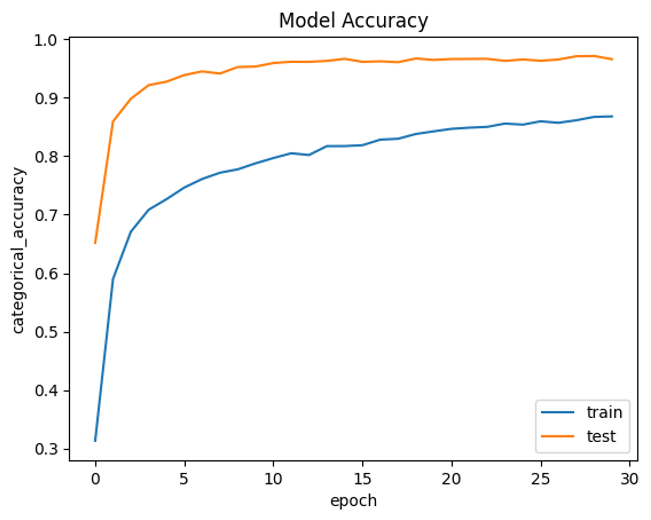
\includegraphics[width=0.7\linewidth]{gambar/bener/Accuracy_ModelResNet50V2.png}
	\captionof{figure}{Akurasi Model CNN ResNet50V2 dengan epoch 30}
	\label{fig:AkurasiCNNResNet50V2}
\end{figure}

Analisis terhadap data akurasi dan validasi akurasi Model CNN ResNet50V2 yang tercantum pada Gambar \ref{fig:AkurasiCNNResNet50V2} menunjukkan perubahan performa model selama 30 epoch pelatihan. Pada awalnya, akurasi model pada data latih memiliki nilai 0.3133944869041443 pada epoch pertama. Namun, seiring berjalannya iterasi pelatihan, terjadi peningkatan yang signifikan dalam akurasi model pada data latih. Pada epoch kedua, terjadi peningkatan yang cukup besar dalam akurasi model menjadi 0.5900458693504333. Penurunan ini menunjukkan bahwa model CNN ResNet50V2 mulai mempelajari pola-pola penting dalam data latih dan mampu menghasilkan prediksi yang lebih akurat. Perubahan ini juga mencerminkan kemampuan model dalam menyesuaikan bobot dan parameter selama pelatihan sebagai upaya meningkatkan performa keseluruhan.

Selanjutnya, pada epoch ke-5, terlihat peningkatan yang lebih lanjut dalam akurasi model dengan nilai 0.72646. Hal ini menandakan adanya kemajuan yang signifikan dalam penyesuaian model dan peningkatan kemampuan model dalam melakukan klasifikasi dengan akurat. Proses iterasi berikutnya juga menunjukkan peningkatan yang stabil dalam akurasi model pada data latih hingga mencapai akurasi tertinggi pada epoch ke-30 dengan nilai 0.868027 .Perubahan akurasi yang terjadi pada model CNN ResNet50V2 mengindikasikan bahwa model tersebut mampu memperbaiki performa klasifikasinya seiring dengan berjalannya waktu dan pelatihan. Penurunan nilai loss yang terjadi sejalan dengan peningkatan akurasi, yang menunjukkan adanya peningkatan kemampuan model dalam menghasilkan prediksi yang sesuai dengan kelas yang ditentukan.

Adanya perubahan yang konsisten dan meningkat dalam akurasi model CNN ResNet50V2 menunjukkan adanya peningkatan yang signifikan dalam kemampuan model dalam mengklasifikasikan data latih. Dalam proses pelatihan, model secara bertahap mempelajari pola-pola klasifikasi yang rumit dan meningkatkan akurasi prediksinya. Dengan kata lain, model CNN ResNet50V2 secara bertahap menjadi lebih akurat dalam mengklasifikasikan data sesuai dengan kelas yang ditentukan.Perubahan akurasi yang terjadi pada model ini menunjukkan bahwa model CNN ResNet50V2 berhasil menyesuaikan diri dengan dataset yang diberikan dan mempelajari pola-pola klasifikasi yang kompleks. Peningkatan akurasi secara bertahap juga menunjukkan bahwa model tidak mengalami overfitting, yaitu kemampuan model mengerjakan generalisasi yang baik pada data yang belum pernah dilihat sebelumnya. Dengan kata lain, model mampu menghasilkan prediksi yang baik pada data baru yang tidak digunakan dalam pelatihan. Selanjutnya, hasil peningkatan akurasi pada data validasi juga menunjukkan kemampuan model CNN ResNet50V2 dalam melakukan generalisasi yang baik. Peningkatan akurasi pada data validasi menunjukkan bahwa model tidak hanya mampu mempelajari pola-pola pada data latih, tetapi juga mampu menghasilkan prediksi yang akurat pada data yang belum pernah dilihat sebelumnya. Secara keseluruhan, analisis terhadap data akurasi dan validasi akurasi Model CNN ResNet50V2 menunjukkan adanya perubahan yang signifikan dalam performa model selama 30 epoch pelatihan. Peningkatan yang konsisten dan meningkat dalam akurasi model pada data latih dan validasi menunjukkan kemampuan model dalam mempelajari pola-pola klasifikasi yang rumit dan menghasilkan prediksi yang akurat.
\begin{figure}[!hbt]
	\centering
	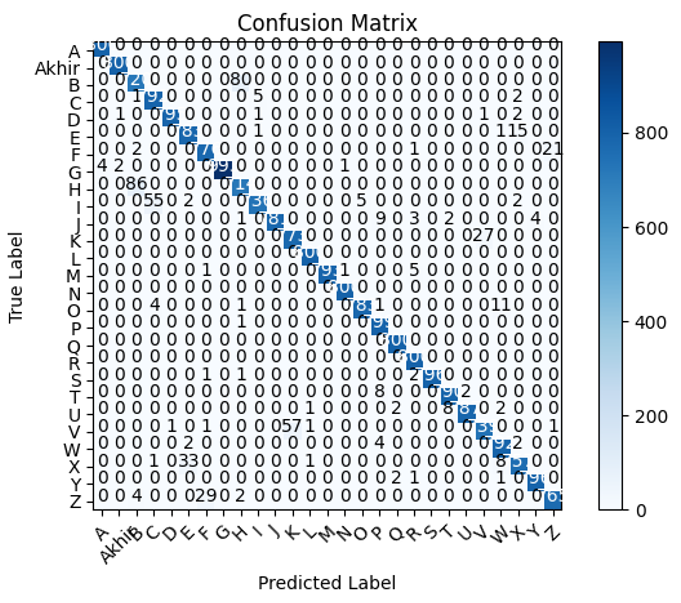
\includegraphics[width=0.7\linewidth]{gambar/bener/ConfusionMatrix_ModelCNNResNet50V2.png}
	\captionof{table}{Hasil Confusion Matriks Model CNN ResNet50V2 dengan epoch 30}
	\label{fig:TabelModelCNNResNet50v2}
\end{figure}
\textit{Confusion Matrix} Model CNN \textit{ResNet50V2} yang terdapat pada Gambar \ref{fig:TabelModelCNNResNet50v2} menunjukkan hasil klasifikasi dari model terhadap setiap kelas dalam dataset. \textit{Confusion Matrix} ini terdiri dari matriks persegi dengan ukuran 27x27, dimana setiap baris mewakili kelas yang sebenarnya dan setiap kolom mewakili kelas yang diprediksi oleh model.Dalam matriks tersebut, nilai pada setiap sel menunjukkan jumlah sampel yang diklasifikasikan dengan benar atau salah oleh model. Sebagai contoh, pada baris pertama dan kolom pertama yang mewakili kelas 'A', terdapat 800 sampel yang diklasifikasikan dengan benar oleh model. Dari hasil \textit{Confusion Matrix}, dapat dilihat bahwa sebagian besar kelas memiliki jumlah sampel yang diklasifikasikan dengan akurat oleh model. Misalnya, pada kelas 'Akhir', tidak ada kesalahan klasifikasi yang terjadi, sehingga semua sampel kelas tersebut diklasifikasikan dengan benar. Namun, terdapat beberapa kesalahan klasifikasi yang terjadi pada beberapa kelas. Sebagai contoh, pada kelas 'G', terdapat 4 sampel yang salah diklasifikasikan sebagai kelas 'A' dan 2 sampel yang salah diklasifikasikan sebagai kelas 'B'. Demikian juga, pada kelas 'E', terdapat 15 sampel yang salah diklasifikasikan sebagai kelas 'X'.

Kesalahan klasifikasi tersebut dapat disebabkan oleh berbagai faktor, seperti kemiripan visual antara kelas yang sulit dibedakan oleh model atau kurangnya representasi data pada kelas tertentu dalam dataset pelatihan. Oleh karena itu, perlu dilakukan analisis lebih lanjut dalam memahami dan mengatasi kesalahan klasifikasi yang terjadi pada kelas-kelas tersebut.Meskipun terdapat kesalahan klasifikasi, secara keseluruhan, model CNN \textit{ResNet50V2} telah menghasilkan performa yang baik dalam melakukan klasifikasi pada dataset ini. Sebagian besar kelas memiliki jumlah sampel yang diklasifikasikan dengan akurat oleh model, sehingga dapat dianggap sebagai prediksi yang dapat diandalkan.
Dalam konteks ini, penting melakukan evaluasi lebih lanjut terhadap kesalahan klasifikasi yang terjadi pada kelas-kelas tertentu. Dengan memahami penyebab kesalahan tersebut, dapat dilakukan langkah-langkah perbaikan seperti peningkatan representasi data atau modifikasi model dengan tujuan meningkatkan performa dalam mengklasifikasikan kelas-kelas yang sulit.

\textit{Confusion Matrix} dapat digunakan sebagai dasar dalam menghitung metrik evaluasi lainnya, seperti precision, recall, dan F1-score bagi setiap kelas. Metrik-metrik tersebut memberikan gambaran yang lebih rinci tentang performa model dalam mengklasifikasikan setiap kelas dan dapat membantu dalam mengidentifikasi area yang perlu diperbaiki.
Dalam kesimpulan, \textit{Confusion Matrix} Model CNN \textit{ResNet50V2} memberikan gambaran tentang hasil klasifikasi model pada dataset. Meskipun terdapat beberapa kesalahan klasifikasi, secara keseluruhan model telah menghasilkan performa yang baik dalam mengklasifikasikan sebagian besar kelas. Analisis lebih lanjut terhadap kesalahan klasifikasi pada kelas tertentu akan membantu meningkatkan performa model dalam tugas klasifikasi pada dataset ini.

Berikut adalah tabel yang menyajikan nilai Precision, Recall, dan F1-Score dari sistem klasifikasi berbagai kelas atau label:

\begin{table}[h]
\centering
\caption{Tabel Evaluasi Metrik CNN ResNet50V2}
\begin{tabular}{|c|c|c|c|c|}
\hline
Class & Precision & Recall & F1-Score \\
\hline
A & 0.995025 & 1.00000 & 0.997506 \\
Akhir & 0.996264 & 1.00000 & 0.998129 \\
B & 0.937500 & 0.90000 & 0.918367 \\
C & 0.930670 & 0.99000 & 0.959419 \\
D & 0.998744 & 0.99375 & 0.996241 \\
E & 0.969059 & 0.97875 & 0.973881 \\
F & 0.960396 & 0.97000 & 0.965174 \\
G & 1.000000 & 0.99300 & 0.996488 \\
H & 0.897375 & 0.94000 & 0.918193 \\
I & 0.990579 & 0.92000 & 0.953986 \\
J & 1.000000 & 0.97625 & 0.987982 \\
K & 0.924101 & 0.86750 & 0.894907 \\
L & 0.996264 & 1.00000 & 0.998129 \\
M & 1.000000 & 0.99125 & 0.995606 \\
N & 0.997506 & 1.00000 & 0.998752 \\
O & 0.993655 & 0.97875 & 0.986146 \\
P & 0.970838 & 0.99875 & 0.984596 \\
Q & 0.995025 & 1.00000 & 0.997506 \\
R & 0.985222 & 1.00000 & 0.992556 \\
S & 1.000000 & 0.99500 & 0.997494 \\
T & 0.987500 & 0.98750 & 0.987500 \\
U & 0.997465 & 0.98375 & 0.990560 \\
V & 0.874556 & 0.92375 & 0.898480 \\
W & 0.974170 & 0.99000 & 0.982021 \\
X & 0.971142 & 0.96750 & 0.969317 \\
Y & 0.995000 & 0.99500 & 0.995000 \\
Z & 0.967130 & 0.95625 & 0.961659 \\
\hline
\end{tabular}
\label{tab:tabelevaluasicnnresnet50v2}
\end{table}

Analisis dari tabel evaluasi metrik pada Tabel \ref{tab:tabelevaluasicnnresnet50v2} memberikan gambaran komprehensif mengenai kinerja sistem klasifikasi bagi setiap kelas atau label yang dievaluasi. Dalam bagian ini dijelaskan lebih detail analisis dari masing-masing parameter metrik, yakni \textit{Precision}, \textit{Recall}, dan \textit{F1-Score}, mulai dari kelas A hingga Z.

Pertama-tama, fokus pertama adalah pada metrik \textit{Precision}. \textit{Precision} mengukur tingkat akurasi sistem dalam mengenali data positif dari seluruh data yang diklasifikasikan sebagai positif. Dari hasil evaluasi, tampak bahwa sebagian besar kelas memiliki tingkat \textit{Precision} yang sangat baik, dengan nilai yang mendekati atau bahkan mencapai 1.00. Hal ini menandakan bahwa sistem memiliki kemampuan yang luar biasa dalam mengenali data positif yang relevan dengan sangat akurat, terutama kelas A, Akhir, D, M, N, Q, dan S. Meskipun begitu, terdapat beberapa kelas seperti H, I, K, V, dan Z yang memiliki tingkat \textit{Precision} yang lebih rendah, sehingga perlu mendapatkan perhatian agar bisa ditingkatkan performanya. Selanjutnya, akan dibahas metrik \textit{Recall}. \textit{Recall} mengukur sejauh mana sistem dapat mengenali seluruh data positif yang ada dari keseluruhan data positif yang sebenarnya. Beberapa kelas, seperti A, Akhir, C, G, J, dan P, menunjukkan nilai \textit{Recall} yang tinggi, mengindikasikan bahwa sistem memiliki kemampuan dalam mengidentifikasi sebagian besar atau bahkan seluruh data positif yang ada. Meskipun begitu, terdapat beberapa kelas lain seperti B, H, I, K, dan V, yang memiliki \textit{Recall} yang lebih rendah, yang menandakan ada potensi  meningkatkan kemampuan sistem dalam mengenali data positif pada kelas-kelas tersebut.

Sekarang, akan ditinjau \textit{F1-Score}. \textit{F1-Score} adalah metrik yang menggabungkan \textit{Precision} dan \textit{Recall}, dan memberikan gambaran keseluruhan tentang performa sistem klasifikasi. Terdapat beberapa kelas yang menonjol dengan \textit{F1-Score} yang tinggi, antara lain kelas A, Akhir, D, M, N, Q, S, dan Z, menandakan bahwa sistem berhasil mencapai keseimbangan yang baik antara \textit{Precision} dan \textit{Recall} bagi kelas-kelas tersebut. Meskipun demikian, beberapa kelas lain seperti B, H, I, K, dan V menunjukkan \textit{F1-Score} yang lebih rendah, yang menjadi fokus utama dalam perbaikan guna meningkatkan performa keseluruhan sistem. Jika melihat rata-rata metrik keseluruhan, dapat disimpulkan bahwa sistem klasifikasi menunjukkan performa yang baik, dengan rata-rata \textit{Precision} sekitar 0.974, \textit{Recall} sekitar 0.978, dan \textit{F1-Score} sekitar 0.975. Hal ini mengindikasikan bahwa sistem secara keseluruhan memiliki kemampuan yang baik dalam mengenali data positif dan mencapai keseimbangan yang optimal antara \textit{Precision} dan \textit{Recall}.

Meskipun hasil evaluasi menunjukkan kinerja yang baik secara keseluruhan, terdapat beberapa kelas yang memerlukan perbaikan performa. Sebagai contoh, kelas H, I, K, dan V menampilkan tingkat Precision, Recall, dan F1-Score yang perlu ditingkatkan. Dengan memfokuskan pada pengembangan dan penyempurnaan sistem kelas-kelas ini, diharapkan akurasi dan efektivitas keseluruhan sistem dapat meningkat secara signifikan.

\section{Model CNN Xception}
Model CNN \textit{Xception} adalah sebuah model \textit{Convolutional Neural Network (CNN)} yang dirancang supaya melakukan klasifikasi gambar pada dataset dengan jumlah kelas yang ditentukan. Model ini menggunakan arsitektur \textit{Xception}, yang sebelumnya telah dilatih pada dataset \textit{ImageNet}. Tujuan dari menggunakan arsitektur \textit{Xception} adalah  memanfaatkan pengetahuan yang telah dipelajari oleh model tersebut dalam mengenali fitur-fitur umum pada gambar. Pada awalnya, model CNN \textit{Xception} menerima input berupa gambar dengan ukuran 128x128 piksel dan 3 \textit{channel} warna \textit{(RGB)}. Kemudian, model \textit{Xception} yang telah dilatih sebelumnya pada \textit{dataset} \textit{ImageNet} dimuat sebagai \textit{base model}. Dalam tahap ini, semua layer pada \textit{base model} dibekukan agar tidak mengalami penyesuaian bobot saat dilatih ulang.

Selanjutnya, \textit{output} dari \textit{base model} digunakan sebagai input lapisan-lapisan selanjutnya dalam model CNN \textit{Xception}. Pertama, \textit{output} dari \textit{base model} diproses melalui lapisan \textit{Flatten} berfungsi sebagai cara meratakan tensor menjadi vektor satu dimensi. Hal ini memungkinkan informasi spasial dari gambar dikonversi menjadi bentuk yang dapat diproses oleh lapisan-lapisan selanjutnya. Kemudian, vektor hasil \textit{flattening} diproses melalui lapisan \textit{Dense} dengan 16 unit \textit{neuron} dan fungsi aktivasi \textit{ReLU}. Fungsi aktivasi \textit{ReLU} membantu dalam memperkenalkan sifat non-linear pada model. Dalam rangka mengurangi overfitting, diterapkan Dropout dengan tingkat dropout sebesar 0.2. Dropout secara acak mengnonaktifkan sejumlah unit \textit{neuron} dalam lapisan tersebut pada setiap iterasi pelatihan.

Selanjutnya, vektor hasil Dropout diproses melalui lapisan \textit{Dense} kedua dengan 16 unit \textit{neuron} dan fungsi aktivasi \textit{ReLU}. Lapisan ini bertujuan memperkuat representasi fitur-fitur yang telah dipelajari sebelumnya. Akhirnya, \textit{output} dari lapisan \textit{Dense} kedua diproses melalui lapisan \textit{Dense} terakhir dengan jumlah unit \textit{neuron} yang sesuai dengan jumlah kelas pada \textit{dataset}. Fungsi aktivasi \textit{softmax} digunakan sebagai cara menghasilkan probabilitas kelas-kelas yang mungkin. Model CNN \textit{Xception} dikompilasi dengan menggunakan fungsi \textit{loss} \textit{mean squared error (MSE)} dan \textit{optimizer} \textit{Adam}. Fungsi \textit{loss} \textit{MSE} digunakan dalam mengukur sejauh mana \textit{output} model berbeda dari label yang sebenarnya pada masalah regresi. Metrik akurasi juga ditentukan agar bisa melacak performa model selama pelatihan. Dalam melakukan pelatihan model, \textit{dataset} yang sesuai dengan jumlah kelas digunakan. Model ini akan belajar mengoptimalkan bobot-bobotnya melalui proses pelatihan dengan harapan dapat mengklasifikasikan gambar-gambar dengan akurasi yang tinggi berdasarkan kelas-kelas yang ditentukan.

\subsection*{Performa dan Fungsionalitas Model CNN \textit{Xception} Skenario Pertama}

Grafik tingkat akurasi dari Model CNN \textit{Xception} dapat ditemukan pada Gambar \ref{fig:akurasiModelCNNXception}. Pada eksperimen ini, model CNN menggunakan arsitektur \textit{Xception} sebagai model dasar. Model CNN ini melalui proses pelatihan selama 30\textit{ epoch}. Grafik tingkat kehilangan (loss) dari Model CNN \textit{Xception} tersedia pada Gambar \ref{fig:lossModelCNNXception}. \textit{Loss} function digunakan sebagai cara mengukur seberapa dekat prediksi model dengan nilai sebenarnya. Dalam eksperimen ini, model CNN berhasil mengurangi tingkat kehilangan secara signifikan selama proses pelatihan selama 30\textit{ epoch}.

\begin{figure}[!hbt]
	\centering
	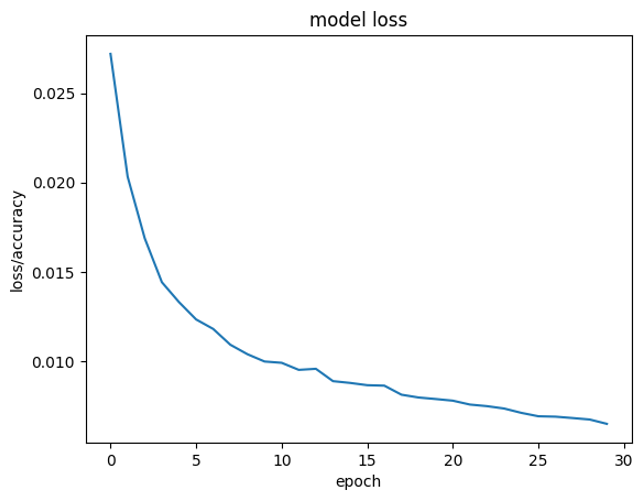
\includegraphics[width=0.7\linewidth]{gambar/bener/Loss_ModelXception.png}
	\captionof{figure}{\textit{Loss} Model CNN Xception dengan epoch 30}
	\label{fig:lossModelCNNXception}
\end{figure}

Analisis terhadap \textit{loss} dari Model CNN \textit{Xception} yang terdapat pada Gambar \ref{fig:lossModelCNNXception} ini menunjukkan tren penurunan yang stabil seiring dengan peningkatan jumlah \textit{epoch}. Pada \textit{epoch} pertama, \textit{loss} awal sebesar 0.027192 . Selanjutnya, \textit{loss} terus menurun pada setiap \textit{epoch} dengan kecenderungan semakin mendekati nol. Pada \textit{epoch} ke-30, \textit{loss} mencapai nilai sebesar 0.00649 . Penurunan \textit{loss} yang konsisten menunjukkan bahwa model CNN \textit{Xception} ini mampu menyesuaikan bobot-bobotnya secara efektif selama pelatihan. Penggunaan arsitektur \textit{Xception} yang telah dilatih pada dataset ImageNet sebagai base model memberikan manfaat dalam mengenali fitur-fitur umum pada gambar, sehingga model dapat dengan lebih baik mempelajari representasi yang relevan terkait tugas klasifikasi yang diberikan. Pada setiap \textit{epoch}, Model CNN \textit{Xception} memperbarui bobot-bobotnya menggunakan optimizer Adam. Optimizer Adam membantu mengoptimalkan bobot-bobot dengan memperhatikan perubahan gradien dan mempercepat konvergensi pelatihan. Dengan demikian, penurunan \textit{loss} yang terjadi pada setiap \textit{epoch} adalah hasil dari pembaruan bobot-bobot tersebut. Secara kuantitatif, penurunan \textit{loss} tersebut menunjukkan bahwa model CNN \textit{Xception} ini semakin mendekati nilai target yaitu nol sesuai yang diinginkan. Semakin kecil nilai loss, semakin baik model dalam melakukan prediksi yang mendekati label yang sebenarnya. Dengan \textit{loss} yang rendah, model ini memiliki kemampuan yang lebih baik dalam mengklasifikasikan gambar-gambar pada dataset dengan akurasi yang tinggi.

Hasil \textit{loss} ini juga dapat digunakan sebagai acuan dalam membandingkan performa model dengan model CNN \textit{Xception} yang lainnya atau dengan model menggunakan arsitektur yang berbeda. Model dengan \textit{loss} yang lebih rendah cenderung memiliki kemampuan yang lebih baik dalam melakukan klasifikasi gambar. Dalam konteks penelitian atau pengembangan lebih lanjut, penurunan \textit{loss} yang signifikan dan konsisten dapat dijadikan indikasi bahwa model CNN \textit{Xception} ini telah melakukan pembelajaran yang baik dan mampu mengekstraksi fitur-fitur yang relevan dari gambar-gambar pada dataset. Secara keseluruhan, penurunan \textit{loss} yang stabil dan konsisten pada Model CNN \textit{Xception} ini menunjukkan kemajuan yang baik dalam pelatihan model. Hasil ini memberikan indikasi bahwa model telah berhasil menyesuaikan bobot-bobotnya dengan baik dan dapat diandalkan dalam melakukan klasifikasi gambar pada dataset yang relevan.

\begin{figure}[!hbt]
	\centering
	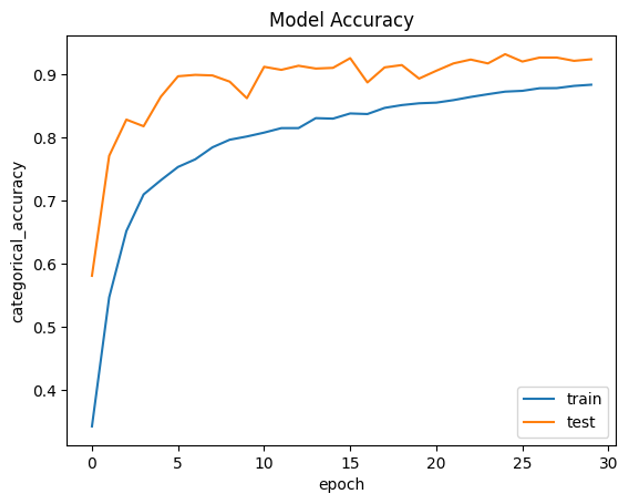
\includegraphics[width=0.7\linewidth]{gambar/bener/Accuracy_ModelXception.png}
	\captionof{figure}{Akurasi Model CNN Xception dengan epoch 30}
	\label{fig:akurasiModelCNNXception}
\end{figure}

Analisis terhadap akurasi dan validasi akurasi dari Model CNN \textit{Xception} pada Gambar \ref{fig:akurasiModelCNNXception} menunjukkan peningkatan yang signifikan seiring dengan jumlah \textit{epoch} yang meningkat. Pada awalnya, akurasi hanya sebesar 0.34197, namun pada \textit{epoch} ke-30, akurasi meningkat menjadi 0.88362. Begitu pula dengan validasi akurasi yang awalnya 0.58074, meningkat menjadi 0.92388 pada \textit{epoch} ke-30.
Penurunan nilai \textit{loss} yang telah dianalisis sebelumnya juga berkontribusi pada peningkatan akurasi dan validasi akurasi. Semakin rendah nilai \textit{loss}, semakin baik model dalam melakukan prediksi yang mendekati label sebenarnya. Dengan demikian, penurunan \textit{loss} memberikan indikasi bahwa model mampu mengenali dan mempelajari pola-pola pada gambar dengan lebih baik.

Dalam konteks perbandingan dengan model-model lain atau arsitektur yang berbeda, hasil akurasi yang tinggi menunjukkan bahwa model CNN \textit{Xception} ini efektif dalam melakukan klasifikasi gambar dengan tingkat keberhasilan yang tinggi. Namun, evaluasi performa model tidak hanya berdasarkan akurasi semata, tetapi juga memperhatikan faktor-faktor lain seperti validasi lintas dan metrik evaluasi lainnya. Selain itu, pengujian pada \textit{dataset} yang berbeda juga perlu dilakukan dalam rangka menguji generalisasi model. Dalam konteks penelitian atau pengembangan lebih lanjut, peningkatan akurasi dan validasi akurasi yang signifikan menunjukkan bahwa model CNN \textit{Xception} ini berhasil dalam pembelajaran dan mampu mengenali pola-pola yang relevan dalam \textit{dataset} gambar. 

Secara keseluruhan, peningkatan akurasi dan validasi akurasi yang signifikan menunjukkan kemajuan yang baik dalam pelatihan model CNN \textit{Xception}. Hasil ini menunjukkan bahwa model mampu menyesuaikan bobot-bobotnya dengan baik dan dapat diandalkan dalam melakukan klasifikasi gambar pada \textit{dataset} yang relevan. Dengan akurasi yang tinggi, model ini memiliki kemampuan yang lebih baik dalam mengklasifikasikan gambar-gambar dengan tingkat keberhasilan yang tinggi. Sebagai bagian dari pengujian fungsionalitas Model CNN Xception, dilakukan perhitungan \textit{Confusion Matrix} . \textit{Confusion Matrix} adalah sebuah matriks yang menampilkan jumlah data yang diklasifikasikan secara benar dan salah dalam setiap kelas. Detail dari \textit{Confusion Matrix} tersebut dapat ditemukan pada Gambar \ref{fig:TabelModelCNNResNet50v2}. Berdasarkan \textit{Confusion Matrix} yang dihasilkan, dilakukan perhitungan beberapa metrik evaluasi seperti \textit{F1-score}, presisi, dan \textit{recall}. Metrik-metrik evaluasi ini memberikan gambaran tentang performa dan akurasi Model CNN dalam melakukan klasifikasi.

\begin{figure}[!hbt]
	\centering
	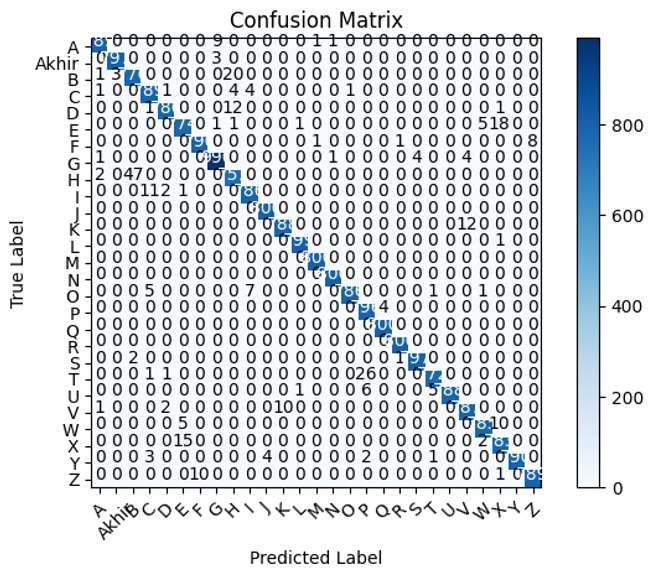
\includegraphics[width=0.7\linewidth]{gambar/bener/ConfusionMatrix_ModelXception.png}
	\captionof{figure}{Confusion Matrix Model CNN Xception dengan epoch 30}
	\label{fig:confusionmatrixModelCNNXception}
\end{figure}

Gambar \ref{fig:confusionmatrixModelCNNXception} \textit{confusion matrix} \textit{Xception}  merupakan representasi dari hasil pengklasifikasian pada Model CNN \textit{Xception}. Matriks tersebut menunjukkan hasil prediksi klasifikasi pada berbagai kelas huruf yang ada. Setiap kolom dan baris pada matriks ini menggambarkan kelas yang diprediksi dan kelas yang sebenarnya. Terdapat 27 kelas huruf yang terklasifikasikan dalam matriks ini.

Pada matriks tersebut, terlihat bahwa terdapat sejumlah hasil yang perlu diperhatikan. Beberapa kelas huruf seperti A, Akhir, F, G, dan M berhasil diklasifikasikan dengan baik oleh model, ditunjukkan oleh nilai \textit{True Positives} yang tinggi. Artinya, model secara akurat mengidentifikasi dan mengklasifikasikan data dengan benar pada kelas-kelas tersebut. Namun, di sisi lain, terdapat beberapa kesalahan prediksi pada beberapa kelas huruf. Misalnya, terdapat kesalahan prediksi pada huruf B, C, D, E, H, dan I, yang ditunjukkan oleh nilai \textit{False Positives} dan \textit{False Negatives} yang ada. Hal ini mengindikasikan bahwa model mengalami kesulitan dalam membedakan dengan tepat antara kelas-kelas tersebut.Pada kelas huruf H dan I, terdapat jumlah \textit{False Positives} yang cukup signifikan, yang menunjukkan kesulitan model dalam membedakan antara kelas tersebut dengan kelas lainnya. Selain itu, kelas huruf B juga mengalami kesulitan dalam pengklasifikasian, ditandai dengan jumlah \textit{False Negatives} dan \textit{False Positives} yang lebih tinggi dibandingkan dengan kelas huruf lainnya. Analisis lebih dalam terhadap matriks ini dapat memberikan wawasan tentang kekuatan dan kelemahan model. Melalui matriks ini, Dapat diidentifikasi kelas huruf mana yang dapat dengan mudah dikenali oleh model dan kelas huruf mana yang menimbulkan kesulitan. Informasi ini penting dalam mengembangkan strategi perbaikan model yang lebih efektif.

Selain itu, matriks \textit{confusion matrix} ini juga dapat digunakan sebagai cara menghitung metrik evaluasi seperti \textit{F1-score}, presisi, dan \textit{recall}. Metrik-metrik ini memberikan gambaran tentang performa dan akurasi Model CNN \textit{Xception} dalam melakukan klasifikasi. Dengan melihat hasil metrik evaluasi, Dapat dievaluasi sejauh mana model ini mampu mengklasifikasikan data dengan benar dan mengukur keberhasilannya dalam mengenali kelas huruf yang berbeda. Secara keseluruhan, matriks \textit{confusion matrix} ini memberikan gambaran tentang kemampuan Model CNN \textit{Xception} dalam melakukan pengklasifikasian huruf-huruf pada dataset. Dengan menganalisis matriks ini,Dapat diidentifikasi kelas huruf yang memerlukan perbaikan lebih lanjut serta memahami kinerja dan kekuatan model secara keseluruhan. Dalam pengembangan model, pemahaman yang mendalam tentang hasil matriks ini dapat digunakan sebagai c ara mengoptimalkan performa model dan meningkatkan akurasi klasifikasi pada dataset yang lebih luas. Perlu diingat bahwa evaluasi model tidak hanya bergantung pada \textit{confusion matrix} semata, tetapi juga melibatkan faktor-faktor lain seperti validasi lintas, analisis kesalahan, dan eksplorasi lebih lanjut terhadap data yang digunakan. Analisis lebih dalam terhadap matriks ini dapat memberikan pandangan yang lebih komprehensif tentang performa model dan memberikan wawasan pengembangan model yang lebih baik di masa depan.

Berikut ini adalah Tabel Evaluasi Metrik dari CNN Xception yang memberikan penjelasan terkait Precision , Recall dan F1-Score dari masing-masing kelas 

\begin{table}[h]
	\centering
	\caption{Tabel Evaluasi Metrik CNN Xception}
	\begin{tabular}{|c|c|c|c|c|}
	\hline
	Kelas & Precision & Recall & F1-Score \\
	\hline
	A & 0.993703 & 0.98625 & 0.989962 \\
	Akhir & 0.993766 & 0.99625 & 0.995006 \\
	B & 0.930456 & 0.97000 & 0.949816 \\
	C & 0.971675 & 0.98625 & 0.978908 \\
	D & 0.963235 & 0.98250 & 0.972772 \\
	E & 0.959108 & 0.96750 & 0.963286 \\
	F & 0.986267 & 0.98750 & 0.986883 \\
	G & 0.986056 & 0.99000 & 0.988024 \\
	H & 0.934744 & 0.66250 & 0.775421 \\
	I & 0.923619 & 0.98250 & 0.952150 \\
	J & 0.990099 & 1.00000 & 0.995025 \\
	K & 0.966033 & 0.88875 & 0.925781 \\
	L & 0.997503 & 0.99875 & 0.998126 \\
	M & 0.997506 & 1.00000 & 0.998752 \\
	N & 0.997506 & 1.00000 & 0.998752 \\
	O & 0.984962 & 0.98250 & 0.983730 \\
	P & 0.874725 & 0.99500 & 0.930994 \\
	Q & 0.995025 & 1.00000 & 0.997506 \\
	R & 0.993789 & 1.00000 & 0.996885 \\
	S & 0.993766 & 0.99625 & 0.995006 \\
	T & 0.991014 & 0.96500 & 0.977834 \\
	U & 1.000000 & 0.98500 & 0.992443 \\
	V & 0.896355 & 0.98375 & 0.938021 \\
	W & 0.967941 & 0.98125 & 0.974550 \\
	X & 0.946250 & 0.94625 & 0.946250 \\
	Y & 1.000000 & 0.98750 & 0.993711 \\
	Z & 0.988722 & 0.98625 & 0.987484 \\
	\hline
	\label{tab:tabelevaluasicnnxception}
	\end{tabular}
	\end{table}

Tabel evaluasi metrik pada Tabel \ref{tab:tabelevaluasicnnxception} memberikan pandangan mendalam tentang kinerja sistem klasifikasi pada berbagai kelas atau label yang dievaluasi. Melalui analisis yang rinci terhadap \textit{Precision}, \textit{Recall}, dan \textit{F1-Score}, kita dapat memahami berbagai aspek penting terkait keakuratan dan keberhasilan sistem dalam melakukan klasifikasi pada masing-masing kelas.

Pertama-tama, \textit{Precision} menggambarkan sejauh mana sistem dapat mengenali positif sejati dengan akurat dari seluruh data yang diklasifikasikan sebagai positif. Hasil evaluasi menunjukkan bahwa sebagian besar kelas memiliki tingkat \textit{Precision} yang sangat baik, dengan nilai mendekati atau bahkan mencapai 1.00. Ini menandakan bahwa sistem memiliki kemampuan yang sangat baik dalam mengidentifikasi data positif yang relevan dari seluruh data yang diklasifikasikan sebagai positif. Beberapa kelas, seperti A, Akhir, D, M, N, Q, dan S, menonjol dengan tingkat \textit{Precision} yang tinggi, sementara beberapa kelas lainnya, seperti H, I, K, V, dan Z, memerlukan peningkatan performa agar mencapai \textit{Precision} yang lebih baik.

Kedua, \textit{Recall} mengukur kemampuan sistem dalam mengenali seluruh data positif yang ada dari seluruh data positif yang sebenarnya. Beberapa kelas, seperti J, M, N, Q, R, dan Y, menampilkan nilai \textit{Recall} yang tinggi, mengindikasikan bahwa sistem memiliki kemampuan dalam mengidentifikasi hampir seluruh data positif yang ada. Namun, terdapat kelas lain, seperti H dan K, yang menampilkan \textit{Recall} yang lebih rendah, menunjukkan adanya potensi dalam meningkatkan kemampuan sistem dalam mengenali data positif pada kelas-kelas tersebut.

Ketiga, \textit{F1-Score} adalah metrik yang menggabungkan \textit{Precision} dan \textit{Recall}, dan memberikan gambaran keseluruhan tentang performa sistem klasifikasi. Beberapa kelas yang menonjol dengan \textit{F1-Score} tinggi adalah L, M, N, Q, dan Z, menandakan bahwa sistem berhasil mencapai keseimbangan yang baik antara \textit{Precision} dan \textit{Recall} pada kelas-kelas tersebut. Meskipun begitu, beberapa kelas lain seperti H, I, K, V, dan X menampilkan \textit{F1-Score} yang lebih rendah, yang menjadi fokus utama perbaikan guna meningkatkan performa keseluruhan sistem.

Rata-rata metrik keseluruhan menunjukkan bahwa sistem klasifikasi menampilkan performa yang baik, dengan nilai rata-rata \textit{Precision} sekitar 0.959, \textit{Recall} sekitar 0.961, dan \textit{F1-Score} sekitar 0.960. Hal ini mengindikasikan bahwa sistem memiliki kemampuan yang memadai dalam mengenali data positif dan mencapai keseimbangan antara \textit{Precision} dan \textit{Recall} secara keseluruhan.

Meskipun hasil evaluasi menunjukkan kinerja yang baik secara keseluruhan, terdapat beberapa kelas yang memerlukan perbaikan performa, khususnya pada aspek \textit{Precision} dan \textit{Recall}. Sebagai contoh, kelas H, I, K, V, dan X menampilkan nilai metrik yang perlu ditingkatkan. Dengan fokus pada pengembangan dan penyempurnaan sistem dari kelas-kelas ini, diharapkan akurasi dan efektivitas keseluruhan sistem dapat meningkat secara signifikan.


\section{Hasil Waktu Pelatihan}
Selain mendapatkan nilai akurasi , \textit{loss} , tabel \textit{Confusion Matrix} , \textit{F1-Score} , \textit{Recall} maupun Presisi . Di dalam penelitian ini juga didapatkan hasil dari lama waktu selama melakukan pelatihan model berbagai macam skenario dari setiap \textit{ epoch} yang berhasil dilewati 

Berikut ini merupakan tabel \ref*{tbl:training_time} yang memaparkan informasi terkait lama waktu pelatihan model per\textit{ epoch} dari masing-masing skenario yang telah diujicoba 
\begin{table}[!hbt]
	\centering
	\captionof{table}{Durasi Pelatihan dalam detik Epoch 1-30}
	\label{tbl:training_time}
	\begin{tabular}{|c|c|c|c|c|} 
	\hline
	Epoch & CNN & CNN2 & Xception & ResNet50V2\\
	\hline
	1              & 18.89        & 19.64         & 212.01            & 200.52              \\
	2              & 19.14        & 19.39         & 204.80            & 208.99              \\
	3              & 18.99        & 18.83         & 210.35            & 201.25              \\
	4              & 18.86        & 19.78         & 214.80            & 191.17              \\
	5              & 19.14        & 20.40         & 201.79            & 195.61              \\
	6              & 20.20        & 20.12         & 202.45            & 192.91              \\
	7              & 19.83        & 19.97         & 198.41            & 192.96              \\
	8              & 21.73        & 19.28         & 192.45            & 191.49              \\
	9              & 20.27        & 20.17         & 189.75            & 196.54              \\
	10             & 19.94        & 20.77         & 188.84            & 199.96              \\
	11             & 20.97        & 21.56         & 189.66            & 195.11              \\
	12             & 21.17        & 20.56         & 187.79            & 188.70              \\
	13             & 21.55        & 20.19         & 188.07            & 189.04              \\
	14             & 21.36        & 20.55         & 185.68            & 224.72              \\
	15             & 21.19        & 19.37         & 184.83            & 208.74              \\
	16             & 21.02        & 20.11         & 185.04            & 217.11              \\
	17             & 21.24        & 20.80         & 188.87            & 204.28              \\
	18             & 21.51        & 19.41         & 190.76            & 224.57              \\
	19             & 21.45        & 19.78         & 193.68            & 204.64              \\
	20             & 21.79        & 19.77         & 193.92            & 181.35              \\
	21             & 20.57        & 19.80         & 186.56            & 175.74              \\
	22             & 21.11        & 20.40         & 185.24            & 180.82              \\
	23             & 21.48        & 20.14         & 185.09            & 173.18              \\
	24             & 21.00        & 20.09         & 186.67            & 163.73              \\
	25             & 21.90        & 20.12         & 185.66            & 168.90              \\
	26             & 23.09        & 20.31         & 185.45            & 164.35              \\
	27             & 22.81        & 19.69         & 184.81            & 164.39              \\
	28             & 23.44        & 19.10         & 185.45            & 163.14              \\
	29             & 22.45        & 19.27         & 187.25            & 161.36              \\
	30             & 22.35        & 19.54         & 187.09            & 162.61              \\ 
	\hline
	\end{tabular}
\end{table}
Tabel \ref{tbl:training_time} menampilkan durasi pelatihan dalam detik bagi masing-masing model, yaitu CNN, CNN2, \textit{Xception}, dan \textit{ResNet50V2}, selama 30 \textit{epoch}. Dalam analisis ini, akan dibahas tentang waktu pelatihan dan perbandingan durasi antara keempat model tersebut.

Pada \textit{epoch} pertama, terlihat bahwa model CNN2 memiliki durasi pelatihan terpendek dengan waktu 19.64 detik, diikuti oleh model CNN dengan waktu 18.89 detik. Model \textit{ResNet50V2} memerlukan waktu pelatihan terlama dengan durasi 200.52 detik, sedangkan model \textit{Xception} memiliki durasi pelatihan sebesar 212.01 detik. Dalam hal ini, durasi pelatihan model CNN2 dan CNN sedikit lebih singkat dibandingkan dengan model \textit{Xception} dan \textit{ResNet50V2}.

Pada \textit{epoch} ke-15, durasi pelatihan Model CNN dan CNN2 masih relatif stabil dengan waktu sekitar 21 detik. Sementara itu, model \textit{Xception} dan \textit{ResNet50V2} memiliki durasi pelatihan yang sedikit berfluktuasi, dengan \textit{Xception} memiliki waktu pelatihan sekitar 185 detik dan \textit{ResNet50V2} sekitar 208 detik. Dalam hal ini, terlihat bahwa model \textit{Xception} memiliki waktu pelatihan yang lebih konsisten dibandingkan dengan model \textit{ResNet50V2}.

Selanjutnya, pada \textit{epoch} ke-30, durasi pelatihan model CNN2 dan CNN tetap stabil dengan waktu sekitar 19-20 detik. Model \textit{Xception} memiliki durasi pelatihan sekitar 187 detik, sedangkan \textit{ResNet50V2} memiliki waktu pelatihan sekitar 162 detik. Dalam hal ini, terlihat bahwa model CNN2 dan CNN mempertahankan waktu pelatihan yang relatif singkat, sedangkan model \textit{Xception} dan \textit{ResNet50V2} tetap dalam kisaran waktu yang lebih lama.

Secara keseluruhan, model CNN2 dan CNN memiliki durasi pelatihan yang relatif singkat, sekitar 19-20 detik, selama 30 \textit{epoch}. Model \textit{Xception} dan \textit{ResNet50V2} memerlukan waktu pelatihan yang lebih lama, dengan \textit{Xception} memiliki durasi pelatihan sekitar 187 detik dan \textit{ResNet50V2} sekitar 162 detik. Perbedaan waktu pelatihan ini dapat disebabkan oleh kompleksitas arsitektur model dan jumlah parameter yang harus dipelajari selama pelatihan.

Dalam konteks ini, model CNN2 dan CNN dapat dianggap sebagai model dengan waktu pelatihan yang lebih efisien dibandingkan dengan model \textit{Xception} dan \textit{ResNet50V2}. Meskipun demikian, faktor-faktor lain seperti performa model dan kebutuhan spesifik tugas dapat menjadi pertimbangan dalam pemilihan model yang paling sesuai.

\section{Ujicoba Deteksi}
Pengujian dilakukan terhadap empat model berbeda, yaitu Model CNN, Model CNN2, ResNet50V2, dan Xception. Model-model tersebut dievaluasi dalam konteks pengenalan pose semaphore yang dihasilkan oleh sembilan koresponden yang berbeda seperti pada Gambar \ref{fig:HasilUjicoba} . Setiap koresponden diminta memperagakan pose semaphore dan menghasilkan lima variasi gerakan setiap huruf dari A hingga E. Pengujian ini dilakukan pada waktu dan lokasi yang berbeda menyesuaikan kondisi dari sembilan koresponden yang mengikuti ujicoba aplikasi 

\begin{figure}[!hbt]
	\centering
	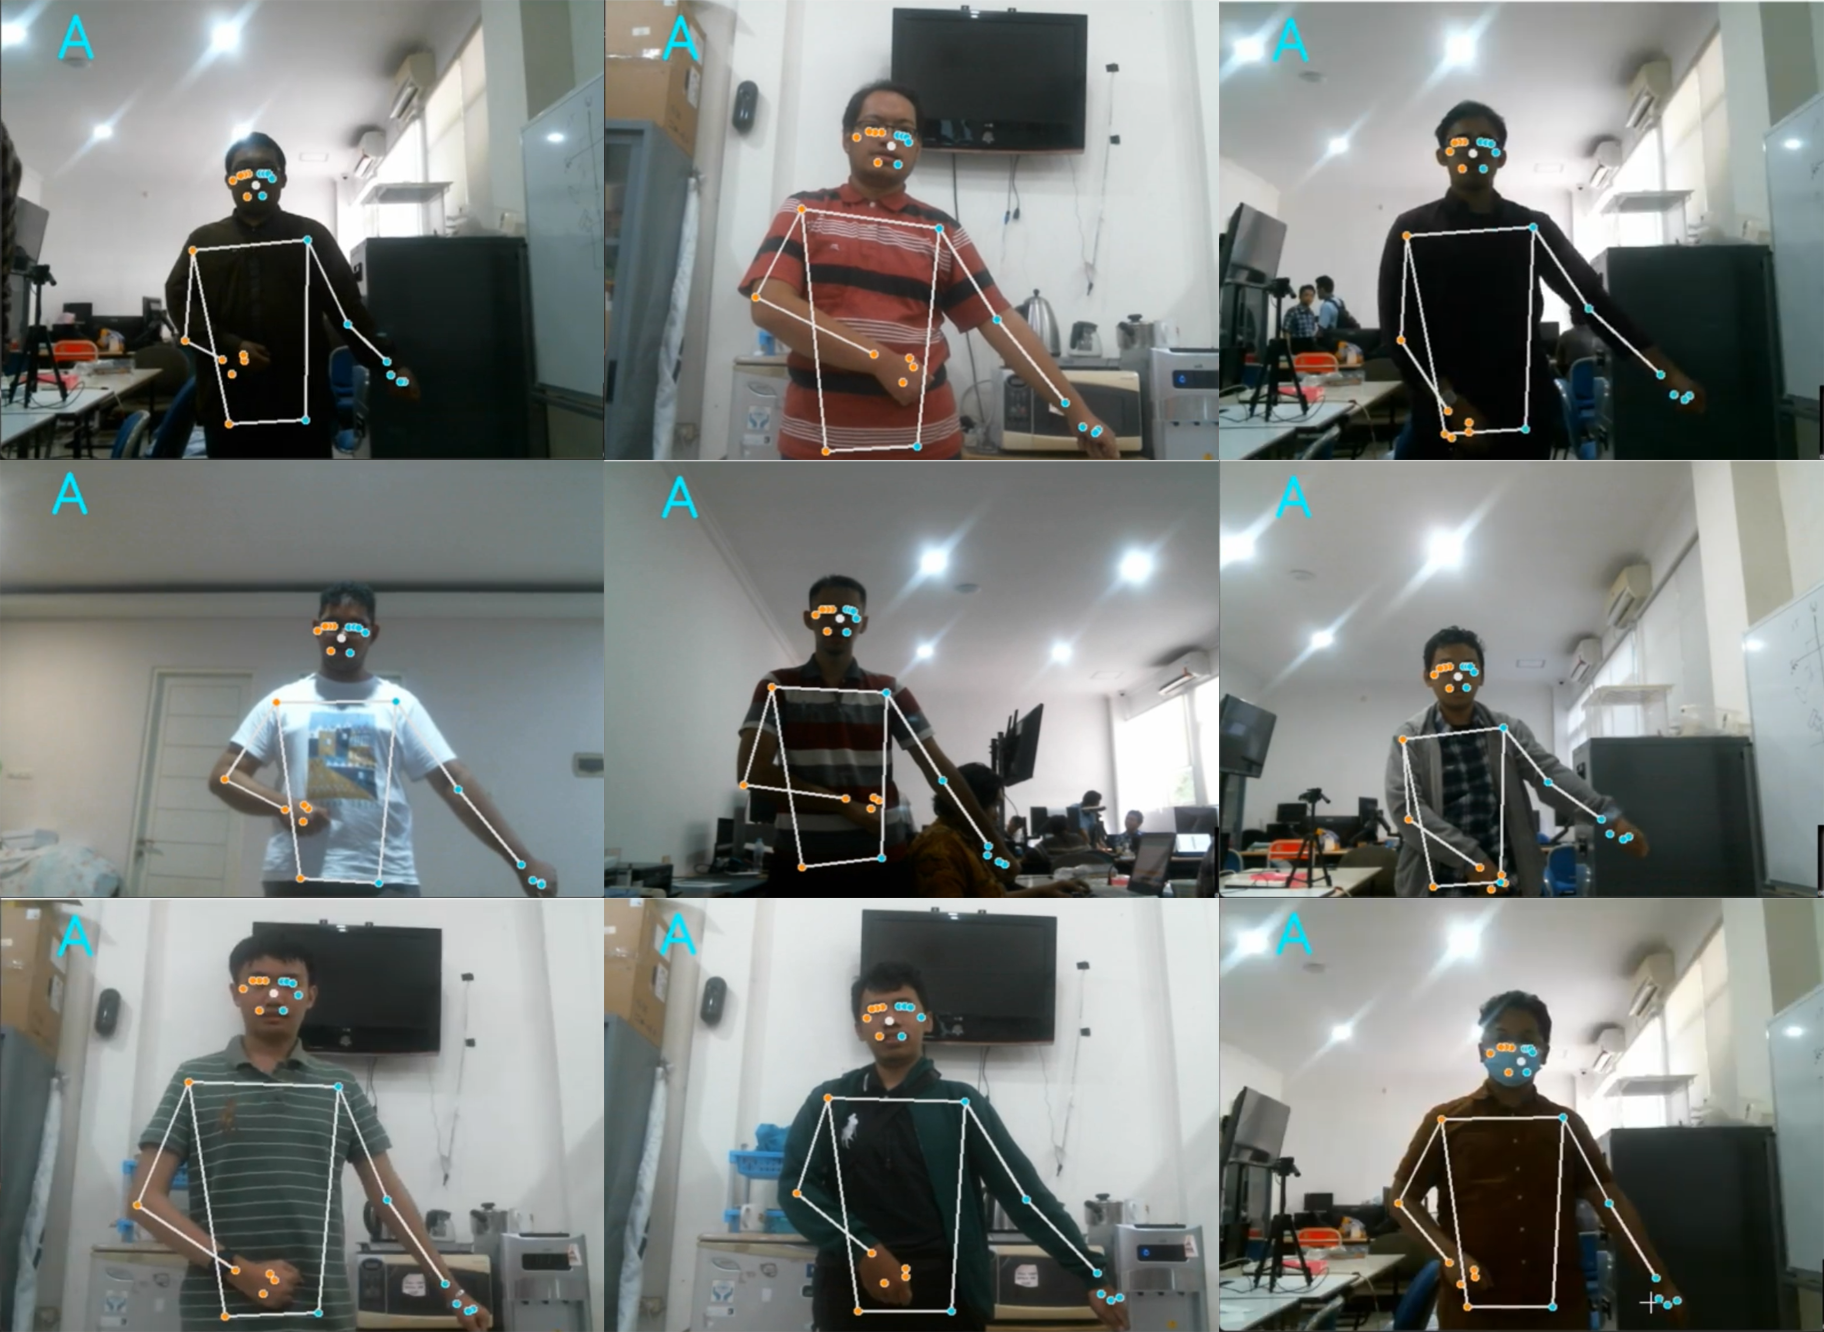
\includegraphics[width=0.7\linewidth]{gambar/bener/Gambar_Ujicoba.png}
	\captionof{figure}{Sembilan Koresponden yang Memperagakan Semaphore Huruf A}
	\label{fig:HasilUjicoba}
\end{figure}

Dalam pengujian ini, proses pengenalan pose semaphore dan variasi gerakan dilakukan oleh aplikasi yang dikembangkan. Aplikasi tersebut mengambil input berupa gambar pose yang dihasilkan oleh para koresponden dan menguji performa dari setiap model. Hasil pengenalan kemudian direkam dan dianalisis agar memahami sejauh mana setiap model dapat mengenali pose semaphore dengan akurasi yang tinggi.

Setiap koresponden menjadi subjek uji coba dalam eksperimen ini, dan mereka secara berurutan diminta  memperagakan pose semaphore dari huruf A hingga E. Proses pengujian dilakukan secara teliti dan cermat agar memastikan variasi gerakan yang berbeda diakuisisi dengan akurat. Hasil pengujian kemudian memberikan pemahaman mendalam tentang efektivitas dan kehandalan setiap model dalam mengenali pose semaphore dan variasi gerakan dari para koresponden yang berpartisipasi. Dengan demikian, pengujian ini memberikan wawasan berharga tentang performa masing-masing model dan dapat menjadi dasar dalam mengoptimalkan dan meningkatkan aplikasi pengenalan pose semaphore di masa mendatang.

Dalam mengujicoba aplikasi pengenalan pose semaphore menggunakan empat model yang berbeda, Juga diterapkan metode evaluasi berdasarkan \textit{confusion matrix}. \textit{Confusion matrix} digunakan sebagai menganalisis performa setiap model dengan lebih rinci dan mendalam. Dengan \textit{confusion matrix}, Dapat dilihat jumlah\textit{ true positive}, \textit{true negative}, \textit{false positive}, dan \textit{false negative} bagi setiap huruf mulai dari A hingga E yang diuji coba. Hasil pengujian juga memberikan informasi penting tentang generalisasi model pada variasi gerakan setiap huruf. Dalam mengenali pose semaphore dari sembilan koresponden yang berbeda, model-model ini menunjukkan performa yang cukup konsisten dalam menghadapi variasi gerakan.

Keseluruhan pengujian ini memberikan gambaran menyeluruh tentang performa dan potensi pengembangan model-model yang digunakan dalam pengenalan pose semaphore. Dengan demikian, penelitian ini memiliki kontribusi signifikan dalam pengembangan sistem klasifikasi yang lebih handal dan efisien untuk aplikasi pengenalan pose semaphore dalam berbagai konteks dan industri.

\section{Hasil Ujicoba Model CNN}
\textit{Confusion Matrix} pada gambar \ref{fig:HasilUjicobaCNN} menggambarkan hasil deteksi huruf A hingga E oleh suatu model. Melalui analisis, diperoleh pemahaman bahwa model berhasil mendeteksi sebagian besar huruf dengan benar, namun tetap mengalami beberapa kesalahan prediksi. Dalam deteksi huruf A, model telah mengidentifikasi 41 huruf A secara tepat, namun terdapat 2 kesalahan prediksi dimana 2 huruf A salah diprediksi sebagai huruf V dan 2 huruf A salah diprediksi sebagai huruf G.

\begin{figure}[!hbt]
	\centering
	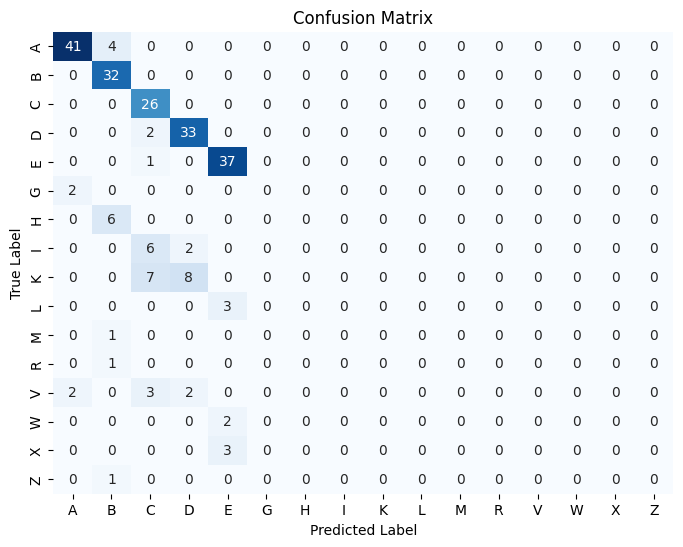
\includegraphics[width=0.7\linewidth]{gambar/bener/ConfusionMatrix-Ujicoba-CNN.png}
	\captionof{figure}{Hasil Confusion Matrix Ujicoba CNN}
	\label{fig:HasilUjicobaCNN}
\end{figure}

Selanjutnya, dalam deteksi huruf B, model juga menunjukkan performa yang baik dengan berhasil mendeteksi 32 huruf B dengan benar. Meskipun demikian, ada 4 kesalahan prediksi di mana 4 huruf B salah diprediksi sebagai huruf A. Kemudian, Dalam melakukan deteksi huruf C, model berhasil mendeteksi 26 huruf C secara benar, namun terdapat beberapa kesalahan prediksi, yaitu 2 huruf C salah diprediksi sebagai huruf D, 1 huruf C salah diprediksi sebagai huruf E, 6 huruf C salah diprediksi sebagai huruf I, dan 7 huruf C salah diprediksi sebagai huruf K.

Selanjutnya, pada deteksi huruf D, model mendeteksi 33 huruf D dengan benar, tetapi masih mengalami beberapa kesalahan prediksi, yaitu 8 huruf D salah diprediksi sebagai huruf K, 2 huruf D salah diprediksi sebagai huruf I, dan 2 huruf D salah diprediksi sebagai huruf V. Terakhir, dalam deteksi huruf E, model berhasil mendeteksi 37 huruf E dengan benar, namun juga terdapat beberapa kesalahan prediksi, di mana 3 huruf E salah diprediksi sebagai huruf L, 2 huruf E salah diprediksi sebagai huruf W, dan 3 huruf E salah diprediksi sebagai huruf X.

\section{Hasil Ujicoba Model CNN2}
\textit{Confusion Matrix} adalah sebuah metode penting yang berfungsi mengevaluasi kinerja suatu model klasifikasi. Seperti pada gambar  \ref{fig:HasilUjicobaCNN2} ,Matriks ini memberikan pandangan mendalam tentang sejauh mana model tersebut berhasil dalam memprediksi kelas yang benar serta seberapa sering kesalahan terjadi dalam proses klasifikasi. Dalam Contoh \textit{Confusion Matrix} di atas, terdapat sepuluh kelas yang harus diprediksi, yaitu A, B, C, D dan E , Mengikuti Hasil Ujicoba dengan Sembilan Koresponden . Setiap kelas memiliki nilai di diagonal matriks yang menunjukkan berapa kali kelas tersebut diprediksi dengan benar oleh model. Selain itu, terdapat pula nilai di luar diagonal yang mencerminkan kesalahan prediksi antar kelas.

\begin{figure}[!hbt]
	\centering
	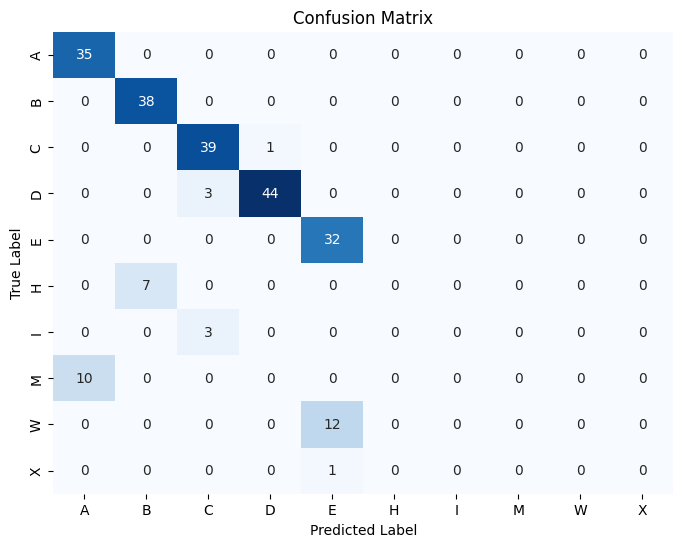
\includegraphics[width=0.7\linewidth]{gambar/bener/ConfusionMatrix-Ujicoba-CNN2.png}
	\captionof{figure}{Hasil Confusion Matrix Ujicoba CNN2}
	\label{fig:HasilUjicobaCNN2}
\end{figure}

Berdasarkan hasil kelas A dalam \textit{Confusion Matrix} tersebut. Kelas A memiliki 35 prediksi positif benar (true positives) dan 10 kesalahan prediksi yang mengarah ke huruf M. Artinya, model telah mengklasifikasikan dengan benar 35 instansi yang termasuk dalam kelas A. Namun, terdapat 10 instansi yang seharusnya termasuk dalam kelas A, tetapi model salah memprediksi sebagai kelas M. Meskipun performa model terhadap kelas A tergolong baik, tetap ada kesalahan yang perlu diperhatikan agar model bisa lebih akurat dalam membedakan kelas A dan M. Kelas B dalam \textit{Confusion Matrix} tersebut. Kelas B memiliki 38 prediksi positif benar \textit{(true positives)} dan 7 kesalahan prediksi yang mengarah ke huruf H. Ini menandakan bahwa model telah berhasil dengan akurat mengklasifikasikan 38 instansi ke dalam kelas B. Namun, terdapat 7 instansi yang seharusnya termasuk dalam kelas B, tetapi model salah memprediksi sebagai kelas H. Meskipun jumlah kesalahan prediksinya terbatas, perlu dilakukan perbaikan dalam rangka meningkatkan akurasi model dalam membedakan kelas B dan H.

Kelas C memiliki 39 prediksi positif benar \textit{(true positives)}, yang menunjukkan bahwa model telah berhasil mengklasifikasikan sebagian besar data yang sebenarnya termasuk dalam kelas C dengan benar. Namun, ada satu kesalahan prediksi di mana model memprediksi satu instansi dari kelas C sebagai kelas D. Kesalahan ini terlihat pada baris ketiga yaitu kelas C dan kolom keempat yaitu kelas D pada \textit{Confusion Matrix}. Meskipun kesalahan ini hanya terjadi pada satu instansi, hal ini tetap perlu diperhatikan agar performa model bisa lebih ditingkatkan lagi. Kelas D menunjukkan performa yang baik dengan 44 prediksi positif benar \textit{(true positives)}. Meskipun begitu, terdapat tiga kesalahan prediksi pada mana model memprediksi tiga instansi dari kelas D sebagai kelas C. Kesalahan ini terlihat pada baris keempat yaitu kelas D dan kolom ketiga yaitu kelas C pada \textit{Confusion Matrix}. Kendati jumlah kesalahan prediksinya terbatas, penting agar memperbaiki kesalahan ini agar kualitas prediksi pada kelas D semakin meningkat.

Kelas E memiliki 32 prediksi positif benar \textit{(true positives)} dan nol kesalahan prediksi. Performa yang sangat baik pada kelas E menandakan bahwa model dengan sangat baik dapat mengenali dan membedakan data yang termasuk ke dalam kelas E. Tidak adanya kesalahan prediksi pada kelas E menunjukkan bahwa model telah dengan tepat mengklasifikasikan seluruh data dari kelas E. Secara keseluruhan, model ini telah berhasil dalam mengklasifikasikan data bagi kelas A hingga E dengan performa yang menggembirakan. Meskipun terdapat beberapa kesalahan dalam melakukan prediksi , model tetap menunjukkan performa yang baik dalam tugas klasifikasinya. 

\section{Hasil Ujicoba Model CNN ResNet50V2}
\textit{Confusion Matrix} pada Gambar  \ref{fig:HasilUjicobaCNNResNet50V2} digunakan sebagai metode evaluasi performa model klasifikasi dengan membandingkan label kelas yang diprediksi dengan label kelas yang sebenarnya. Dalam kasus ini, \textit{Confusion Matrix} mewakili hasil evaluasi model klasifikasi pada sembilan koresponden, di mana setiap baris mewakili label kelas sebenarnya, dan setiap kolom mewakili label kelas yang diprediksi dari kelas A hingga E. Pada paragraf pertama, Dapat dilihat performa model pada kelas A. Dari 41 contoh yang termasuk kelas A, model berhasil memprediksi semuanya dengan benar, tanpa ada false negative dan false positive. Ini menunjukkan bahwa model memiliki akurasi tinggi dalam mengklasifikasikan contoh-contoh kelas A. Namun, penting agar mempertimbangkan ketidakseimbangan kelas, karena jumlah contoh pada kelas A jauh lebih sedikit dibandingkan dengan kelas lainnya.

\begin{figure}[!hbt]
	\centering
	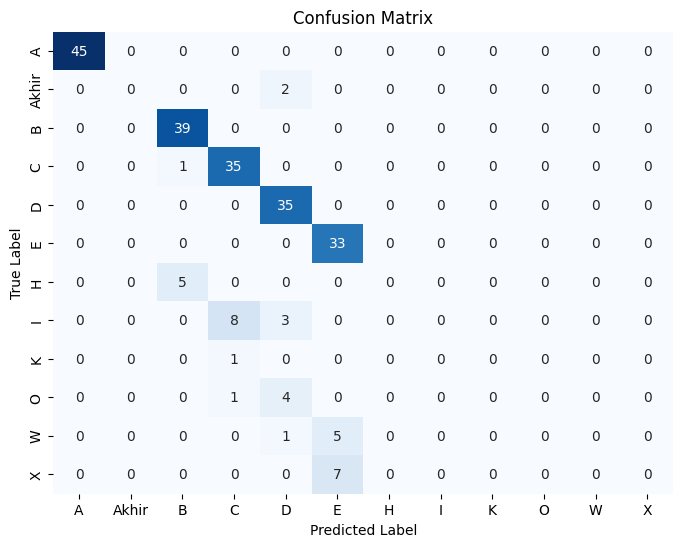
\includegraphics[width=0.7\linewidth]{gambar/bener/ConfusionMatrix-Ujicoba-ResNet50V2.png}
	\captionof{figure}{Hasil Confusion Matrix Ujicoba CNN ResNet50V2}
	\label{fig:HasilUjicobaCNNResNet50V2}
\end{figure}

Beralih ke kelas B, terdapat 32 contoh kelas B, dan model berhasil mengklasifikasikan semuanya dengan benar. Seperti pada kelas A, tidak ada false negative dan false positive. Sekali lagi, ini menunjukkan performa yang tinggi dalam memprediksi contoh-contoh kelas B, tetapi ketidakseimbangan kelas bisa menjadi perhatian. Kelas C memiliki 26 contoh, dan model berhasil mengklasifikasikan semuanya dengan benar. Seperti pada kelas A dan B, tidak ada false negative dan false positive. Ini menunjukkan performa yang sangat baik dalam mengklasifikasikan contoh-contoh kelas C, tetapi masalah ketidakseimbangan kelas tetap ada. Kelas D memiliki 33 contoh, dan model berhasil mengklasifikasikan 33 contoh tersebut dengan benar, tanpa adanya false negative. Namun, ada 2 false positive, menunjukkan bahwa model salah mengklasifikasikan dua contoh sebagai kelas D padahal sebenarnya termasuk kelas lain. Performa keseluruhan pada kelas D masih cukup baik, tetapi false positive mengindikasikan ada ruang perbaikan. Beralih ke kelas E, yang memiliki 37 contoh, model berhasil mengklasifikasikan semuanya dengan benar, tanpa false negative. Seperti pada kelas D, terdapat 1 false positive, menunjukkan bahwa satu contoh salah diklasifikasikan sebagai kelas E. Secara keseluruhan, performa model pada kelas E cukup baik, namun seperti kelas D, ada sedikit masalah dengan false positive.

Secara keseluruhan, model menunjukkan performa yang sangat baik pada kelas A hingga E, dengan mengklasifikasikan sebagian besar contoh pada setiap kelas dengan benar. Namun, adanya false positive pada kelas D dan E menunjukkan ada ruang perbaikan. Selain itu, ketidakseimbangan kelas pada kelas A, B, dan C juga harus dipertimbangkan saat mengevaluasi performa keseluruhan model.

\section{Hasil Ujicoba Model CNN Xception}
\textit{Confusion matrix} yang ditampilkan pada Gambar  \ref{fig:HasilUjicobaCNNXception} merepresentasikan evaluasi kinerja model prediksi dalam sistem semaphore menggunakan model CNN \textit{Xception}. Perlu dicatat bahwa data yang digunakan berasal dari sembilan koresponden yang berbeda. Dalam evaluasi ini, Dapat dilihat bahwa prediksi huruf A memiliki tingkat akurasi yang baik, di mana 41 data berhasil diidentifikasi dengan benar sebagai huruf A \textit{(true positive)}. Namun, ada 2 data yang keliru diprediksi sebagai huruf G \textit{(false positive)}, dan beberapa data G yang seharusnya termasuk huruf A diprediksi sebagai G \textit{(false negative)}. Oleh karena itu, model perlu ditingkatkan dalam membedakan antara huruf A dan G.

\begin{figure}[!hbt]
	\centering
	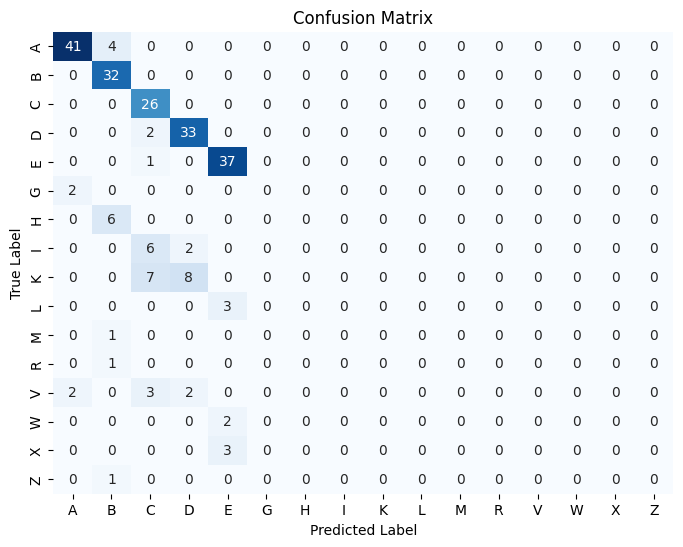
\includegraphics[width=0.7\linewidth]{gambar/bener/ConfusionMatrix-Ujicoba-Xception.png}
	\captionof{figure}{Hasil Confusion Matrix Ujicoba CNN Xception}
	\label{fig:HasilUjicobaCNNXception}
\end{figure}

Hasil evaluasi juga menunjukkan kinerja yang sangat baik pada klasifikasi huruf B dan C. Model berhasil memprediksi 32 data sebagai huruf B dengan benar \textit{(true positive)} dan 26 data sebagai huruf C dengan tepat \textit{(true positive)}. Tidak ada kesalahan prediksi pada huruf-huruf ini (false positive dan false negative). Hal ini menunjukkan bahwa model memiliki kemampuan yang handal dalam mengenali huruf B dan C.

Namun, terdapat beberapa kesalahan dalam klasifikasi huruf D dan E. Model berhasil memprediksi 33 data sebagai huruf D dengan benar \textit{(true positive)}, namun beberapa data huruf K keliru diprediksi sebagai huruf D \textit{(false positive)}, dan sebaliknya, ada beberapa data huruf D yang keliru diprediksi sebagai huruf K \textit{(false negative)}. Hal serupa terjadi pada huruf E, di mana model berhasil memprediksi 37 data dengan benar \textit{(true positive)}, tetapi ada satu data huruf C yang keliru diprediksi sebagai huruf E \textit{(false positive)}, dan beberapa data huruf C diprediksi sebagai huruf E \textit{(false negative)}.